%% bare_jrnl.tex
%% V1.4b
%% 2015/08/26
%% by Michael Shell
%% see http://www.michaelshell.org/
%% for current contact information.
%%
%% This is a skeleton file demonstrating the use of IEEEtran.cls
%% (requires IEEEtran.cls version 1.8b or later) with an IEEE
%% journal paper.
%%
%% Support sites:
%% http://www.michaelshell.org/tex/ieeetran/
%% http://www.ctan.org/pkg/ieeetran
%% and
%% http://www.ieee.org/

%%*************************************************************************
%% Legal Notice:
%% This code is offered as-is without any warranty either expressed or
%% implied; without even the implied warranty of MERCHANTABILITY or
%% FITNESS FOR A PARTICULAR PURPOSE! 
%% User assumes all risk.
%% In no event shall the IEEE or any contributor to this code be liable for
%% any damages or losses, including, but not limited to, incidental,
%% consequential, or any other damages, resulting from the use or misuse
%% of any information contained here.
%%
%% All comments are the opinions of their respective authors and are not
%% necessarily endorsed by the IEEE.
%%
%% This work is distributed under the LaTeX Project Public License (LPPL)
%% ( http://www.latex-project.org/ ) version 1.3, and may be freely used,
%% distributed and modified. A copy of the LPPL, version 1.3, is included
%% in the base LaTeX documentation of all distributions of LaTeX released
%% 2003/12/01 or later.
%% Retain all contribution notices and credits.
%% ** Modified files should be clearly indicated as such, including  **
%% ** renaming them and changing author support contact information. **
%%*************************************************************************


% *** Authors should verify (and, if needed, correct) their LaTeX system  ***
% *** with the testflow diagnostic prior to trusting their LaTeX platform ***
% *** with production work. The IEEE's font choices and paper sizes can   ***
% *** trigger bugs that do not appear when using other class files.       ***                          ***
% The testflow support page is at:
% http://www.michaelshell.org/tex/testflow/



\documentclass[journal]{IEEEtran}
%
% If IEEEtran.cls has not been installed into the LaTeX system files,
% manually specify the path to it like:
% \documentclass[journal]{../sty/IEEEtran}

\usepackage{enumerate}  
\newcommand{\RNum}[1]{\uppercase\expandafter{\romannumeral #1\relax}}
\usepackage{amsmath}
\usepackage{algorithm}  
\usepackage{algorithmic}
\usepackage{enumerate}  
\usepackage{amsmath}
\usepackage{graphicx} 
\usepackage{amssymb}
\usepackage{subfigure}

% Some very useful LaTeX packages include:
% (uncomment the ones you want to load)


% *** MISC UTILITY PACKAGES ***
%
%\usepackage{ifpdf}
% Heiko Oberdiek's ifpdf.sty is very useful if you need conditional
% compilation based on whether the output is pdf or dvi.
% usage:
% \ifpdf
%   % pdf code
% \else
%   % dvi code
% \fi
% The latest version of ifpdf.sty can be obtained from:
% http://www.ctan.org/pkg/ifpdf
% Also, note that IEEEtran.cls V1.7 and later provides a builtin
% \ifCLASSINFOpdf conditional that works the same way.
% When switching from latex to pdflatex and vice-versa, the compiler may
% have to be run twice to clear warning/error messages.






% *** CITATION PACKAGES ***
%
%\usepackage{cite}
% cite.sty was written by Donald Arseneau
% V1.6 and later of IEEEtran pre-defines the format of the cite.sty package
% \cite{} output to follow that of the IEEE. Loading the cite package will
% result in citation numbers being automatically sorted and properly
% "compressed/ranged". e.g., [1], [9], [2], [7], [5], [6] without using
% cite.sty will become [1], [2], [5]--[7], [9] using cite.sty. cite.sty's
% \cite will automatically add leading space, if needed. Use cite.sty's
% noadjust option (cite.sty V3.8 and later) if you want to turn this off
% such as if a citation ever needs to be enclosed in parenthesis.
% cite.sty is already installed on most LaTeX systems. Be sure and use
% version 5.0 (2009-03-20) and later if using hyperref.sty.
% The latest version can be obtained at:
% http://www.ctan.org/pkg/cite
% The documentation is contained in the cite.sty file itself.






% *** GRAPHICS RELATED PACKAGES ***
%
\ifCLASSINFOpdf
  % \usepackage[pdftex]{graphicx}
  % declare the path(s) where your graphic files are
  % \graphicspath{{../pdf/}{../jpeg/}}
  % and their extensions so you won't have to specify these with
  % every instance of \includegraphics
  % \DeclareGraphicsExtensions{.pdf,.jpeg,.png}
\else
  % or other class option (dvipsone, dvipdf, if not using dvips). graphicx
  % will default to the driver specified in the system graphics.cfg if no
  % driver is specified.
  % \usepackage[dvips]{graphicx}
  % declare the path(s) where your graphic files are
  % \graphicspath{{../eps/}}
  % and their extensions so you won't have to specify these with
  % every instance of \includegraphics
  % \DeclareGraphicsExtensions{.eps}
\fi
% graphicx was written by David Carlisle and Sebastian Rahtz. It is
% required if you want graphics, photos, etc. graphicx.sty is already
% installed on most LaTeX systems. The latest version and documentation
% can be obtained at: 
% http://www.ctan.org/pkg/graphicx
% Another good source of documentation is "Using Imported Graphics in
% LaTeX2e" by Keith Reckdahl which can be found at:
% http://www.ctan.org/pkg/epslatex
%
% latex, and pdflatex in dvi mode, support graphics in encapsulated
% postscript (.eps) format. pdflatex in pdf mode supports graphics
% in .pdf, .jpeg, .png and .mps (metapost) formats. Users should ensure
% that all non-photo figures use a vector format (.eps, .pdf, .mps) and
% not a bitmapped formats (.jpeg, .png). The IEEE frowns on bitmapped formats
% which can result in "jaggedy"/blurry rendering of lines and letters as
% well as large increases in file sizes.
%
% You can find documentation about the pdfTeX application at:
% http://www.tug.org/applications/pdftex





% *** MATH PACKAGES ***
%
%\usepackage{amsmath}
% A popular package from the American Mathematical Society that provides
% many useful and powerful commands for dealing with mathematics.
%
% Note that the amsmath package sets \interdisplaylinepenalty to 10000
% thus preventing page breaks from occurring within multiline equations. Use:
%\interdisplaylinepenalty=2500
% after loading amsmath to restore such page breaks as IEEEtran.cls normally
% does. amsmath.sty is already installed on most LaTeX systems. The latest
% version and documentation can be obtained at:
% http://www.ctan.org/pkg/amsmath





% *** SPECIALIZED LIST PACKAGES ***
%
%\usepackage{algorithmic}
% algorithmic.sty was written by Peter Williams and Rogerio Brito.
% This package provides an algorithmic environment fo describing algorithms.
% You can use the algorithmic environment in-text or within a figure
% environment to provide for a floating algorithm. Do NOT use the algorithm
% floating environment provided by algorithm.sty (by the same authors) or
% algorithm2e.sty (by Christophe Fiorio) as the IEEE does not use dedicated
% algorithm float types and packages that provide these will not provide
% correct IEEE style captions. The latest version and documentation of
% algorithmic.sty can be obtained at:
% http://www.ctan.org/pkg/algorithms
% Also of interest may be the (relatively newer and more customizable)
% algorithmicx.sty package by Szasz Janos:
% http://www.ctan.org/pkg/algorithmicx




% *** ALIGNMENT PACKAGES ***
%
%\usepackage{array}
% Frank Mittelbach's and David Carlisle's array.sty patches and improves
% the standard LaTeX2e array and tabular environments to provide better
% appearance and additional user controls. As the default LaTeX2e table
% generation code is lacking to the point of almost being broken with
% respect to the quality of the end results, all users are strongly
% advised to use an enhanced (at the very least that provided by array.sty)
% set of table tools. array.sty is already installed on most systems. The
% latest version and documentation can be obtained at:
% http://www.ctan.org/pkg/array


% IEEEtran contains the IEEEeqnarray family of commands that can be used to
% generate multiline equations as well as matrices, tables, etc., of high
% quality.




% *** SUBFIGURE PACKAGES ***
%\ifCLASSOPTIONcompsoc
%  \usepackage[caption=false,font=normalsize,labelfont=sf,textfont=sf]{subfig}
%\else
%  \usepackage[caption=false,font=footnotesize]{subfig}
%\fi
% subfig.sty, written by Steven Douglas Cochran, is the modern replacement
% for subfigure.sty, the latter of which is no longer maintained and is
% incompatible with some LaTeX packages including fixltx2e. However,
% subfig.sty requires and automatically loads Axel Sommerfeldt's caption.sty
% which will override IEEEtran.cls' handling of captions and this will result
% in non-IEEE style figure/table captions. To prevent this problem, be sure
% and invoke subfig.sty's "caption=false" package option (available since
% subfig.sty version 1.3, 2005/06/28) as this is will preserve IEEEtran.cls
% handling of captions.
% Note that the Computer Society format requires a larger sans serif font
% than the serif footnote size font used in traditional IEEE formatting
% and thus the need to invoke different subfig.sty package options depending
% on whether compsoc mode has been enabled.
%
% The latest version and documentation of subfig.sty can be obtained at:
% http://www.ctan.org/pkg/subfig




% *** FLOAT PACKAGES ***
%
%\usepackage{fixltx2e}
% fixltx2e, the successor to the earlier fix2col.sty, was written by
% Frank Mittelbach and David Carlisle. This package corrects a few problems
% in the LaTeX2e kernel, the most notable of which is that in current
% LaTeX2e releases, the ordering of single and double column floats is not
% guaranteed to be preserved. Thus, an unpatched LaTeX2e can allow a
% single column figure to be placed prior to an earlier double column
% figure.
% Be aware that LaTeX2e kernels dated 2015 and later have fixltx2e.sty's
% corrections already built into the system in which case a warning will
% be issued if an attempt is made to load fixltx2e.sty as it is no longer
% needed.
% The latest version and documentation can be found at:
% http://www.ctan.org/pkg/fixltx2e


%\usepackage{stfloats}
% stfloats.sty was written by Sigitas Tolusis. This package gives LaTeX2e
% the ability to do double column floats at the bottom of the page as well
% as the top. (e.g., "\begin{figure*}[!b]" is not normally possible in
% LaTeX2e). It also provides a command:
%\fnbelowfloat
% to enable the placement of footnotes below bottom floats (the standard
% LaTeX2e kernel puts them above bottom floats). This is an invasive package
% which rewrites many portions of the LaTeX2e float routines. It may not work
% with other packages that modify the LaTeX2e float routines. The latest
% version and documentation can be obtained at:
% http://www.ctan.org/pkg/stfloats
% Do not use the stfloats baselinefloat ability as the IEEE does not allow
% \baselineskip to stretch. Authors submitting work to the IEEE should note
% that the IEEE rarely uses double column equations and that authors should try
% to avoid such use. Do not be tempted to use the cuted.sty or midfloat.sty
% packages (also by Sigitas Tolusis) as the IEEE does not format its papers in
% such ways.
% Do not attempt to use stfloats with fixltx2e as they are incompatible.
% Instead, use Morten Hogholm'a dblfloatfix which combines the features
% of both fixltx2e and stfloats:
%
% \usepackage{dblfloatfix}
% The latest version can be found at:
% http://www.ctan.org/pkg/dblfloatfix




%\ifCLASSOPTIONcaptionsoff
%  \usepackage[nomarkers]{endfloat}
% \let\MYoriglatexcaption\caption
% \renewcommand{\caption}[2][\relax]{\MYoriglatexcaption[#2]{#2}}
%\fi
% endfloat.sty was written by James Darrell McCauley, Jeff Goldberg and 
% Axel Sommerfeldt. This package may be useful when used in conjunction with 
% IEEEtran.cls'  captionsoff option. Some IEEE journals/societies require that
% submissions have lists of figures/tables at the end of the paper and that
% figures/tables without any captions are placed on a page by themselves at
% the end of the document. If needed, the draftcls IEEEtran class option or
% \CLASSINPUTbaselinestretch interface can be used to increase the line
% spacing as well. Be sure and use the nomarkers option of endfloat to
% prevent endfloat from "marking" where the figures would have been placed
% in the text. The two hack lines of code above are a slight modification of
% that suggested by in the endfloat docs (section 8.4.1) to ensure that
% the full captions always appear in the list of figures/tables - even if
% the user used the short optional argument of \caption[]{}.
% IEEE papers do not typically make use of \caption[]'s optional argument,
% so this should not be an issue. A similar trick can be used to disable
% captions of packages such as subfig.sty that lack options to turn off
% the subcaptions:
% For subfig.sty:
% \let\MYorigsubfloat\subfloat
% \renewcommand{\subfloat}[2][\relax]{\MYorigsubfloat[]{#2}}
% However, the above trick will not work if both optional arguments of
% the \subfloat command are used. Furthermore, there needs to be a
% description of each subfigure *somewhere* and endfloat does not add
% subfigure captions to its list of figures. Thus, the best approach is to
% avoid the use of subfigure captions (many IEEE journals avoid them anyway)
% and instead reference/explain all the subfigures within the main caption.
% The latest version of endfloat.sty and its documentation can obtained at:
% http://www.ctan.org/pkg/endfloat
%
% The IEEEtran \ifCLASSOPTIONcaptionsoff conditional can also be used
% later in the document, say, to conditionally put the References on a 
% page by themselves.




% *** PDF, URL AND HYPERLINK PACKAGES ***
%
%\usepackage{url}
% url.sty was written by Donald Arseneau. It provides better support for
% handling and breaking URLs. url.sty is already installed on most LaTeX
% systems. The latest version and documentation can be obtained at:
% http://www.ctan.org/pkg/url
% Basically, \url{my_url_here}.




% *** Do not adjust lengths that control margins, column widths, etc. ***
% *** Do not use packages that alter fonts (such as pslatex).         ***
% There should be no need to do such things with IEEEtran.cls V1.6 and later.
% (Unless specifically asked to do so by the journal or conference you plan
% to submit to, of course. )


% correct bad hyphenation here
\hyphenation{op-tical net-works semi-conduc-tor}


\begin{document}
%
% paper title
% Titles are generally capitalized except for words such as a, an, and, as,
% at, but, by, for, in, nor, of, on, or, the, to and up, which are usually
% not capitalized unless they are the first or last word of the title.
% Linebreaks \\ can be used within to get better formatting as desired.
% Do not put math or special symbols in the title.
\title{Bare Demo of IEEEtran.cls\\ for IEEE Journals}
%
%
% author names and IEEE memberships
% note positions of commas and nonbreaking spaces ( ~ ) LaTeX will not break
% a structure at a ~ so this keeps an author's name from being broken across
% two lines.
% use \thanks{} to gain access to the first footnote area
% a separate \thanks must be used for each paragraph as LaTeX2e's \thanks
% was not built to handle multiple paragraphs
%

\author{Michael~Shell,~\IEEEmembership{Member,~IEEE,}
        John~Doe,~\IEEEmembership{Fellow,~OSA,}
        and~Jane~Doe,~\IEEEmembership{Life~Fellow,~IEEE}% <-this % stops a space
}

% note the % following the last \IEEEmembership and also \thanks - 
% these prevent an unwanted space from occurring between the last author name
% and the end of the author line. i.e., if you had this:
% 
% \author{....lastname \thanks{...} \thanks{...} }
%                     ^------------^------------^----Do not want these spaces!
%
% a space would be appended to the last name and could cause every name on that
% line to be shifted left slightly. This is one of those "LaTeX things". For
% instance, "\textbf{A} \textbf{B}" will typeset as "A B" not "AB". To get
% "AB" then you have to do: "\textbf{A}\textbf{B}"
% \thanks is no different in this regard, so shield the last } of each \thanks
% that ends a line with a % and do not let a space in before the next \thanks.
% Spaces after \IEEEmembership other than the last one are OK (and needed) as
% you are supposed to have spaces between the names. For what it is worth,
% this is a minor point as most people would not even notice if the said evil
% space somehow managed to creep in.



% The paper headers
\markboth{Journal of \LaTeX\ Class Files,~Vol.~14, No.~8, August~2015}%
{Shell \MakeLowercase{\textit{et al.}}: Bare Demo of IEEEtran.cls for IEEE Journals}
% The only time the second header will appear is for the odd numbered pages
% after the title page when using the twoside option.
% 
% *** Note that you probably will NOT want to include the author's ***
% *** name in the headers of peer review papers.                   ***
% You can use \ifCLASSOPTIONpeerreview for conditional compilation here if
% you desire.




% If you want to put a publisher's ID mark on the page you can do it like
% this:
%\IEEEpubid{0000--0000/00\$00.00~\copyright~2015 IEEE}
% Remember, if you use this you must call \IEEEpubidadjcol in the second
% column for its text to clear the IEEEpubid mark.



% use for special paper notices
%\IEEEspecialpapernotice{(Invited Paper)}




% make the title area
\maketitle

% As a general rule, do not put math, special symbols or citations
% in the abstract or keywords.
\begin{abstract}
With the emergence of advanced vehicular service, the challenge of meeting computation and communication needs of vehicles has become increasingly prominent. Computation offloading is a promising paradigm to .
\end{abstract}

% Note that keywords are not normally used for peerreview papers.
\begin{IEEEkeywords}
Fog Computing, Computation offloading, Vehicular Network, Workload Allocation
\end{IEEEkeywords}






% For peer review papers, you can put extra information on the cover
% page as needed:
% \ifCLASSOPTIONpeerreview
% \begin{center} \bfseries EDICS Category: 3-BBND \end{center}
% \fi
%
% For peerreview papers, this IEEEtran command inserts a page break and
% creates the second title. It will be ignored for other modes.
\IEEEpeerreviewmaketitle



\section{Introduction}
% The very first letter is a 2 line initial drop letter followed
% by the rest of the first word in caps.
% 
% form to use if the first word consists of a single letter:
% \IEEEPARstart{A}{demo} file is ....
% 
% form to use if you need the single drop letter followed by
% normal text (unknown if ever used by the IEEE):
% \IEEEPARstart{A}{}demo file is ....
% 
% Some journals put the first two words in caps:
% \IEEEPARstart{T}{his demo} file is ....
% 
% Here we have the typical use of a "T" for an initial drop letter
% and "HIS" in caps to complete the first word.
\IEEEPARstart{W}ith the development of Internet of Things(IoT) and wireless technologies, vehicles become more intelligent and provide better services\cite{1}. In this process, various complex-computing applications such as autonomous driving and image recognition are required to meet the demands of users. However, the computation limitation of vehicle terminal make it difficult to meet these demands and many advanced applications cannot be applied on vehicles.Without powerful computational support, various applications are still in the concept phase and cannot be applied in our daily life\cite{2},\cite{3}.

Cloud computing can improve the computation performance by offloading tasks to the cloud which takes the advantage of abundant computational resource\cite{4}. However, the long distance transmission of data to cloud has not only caused a heavy burden on communication links but also resulted in intolerable latency, which significantly degrades the QoS. To overcome the above problem, fog computing is a new paradigm extending the computation facilities to the user end \cite{5},\cite{6}. This paradigm is a promising method to solve the computation limitation of vehicle \cite{7}. On the one hand, the fog device reduce the power consumption by relieving the workload of cloud. On the other hand, the geo-distributed fog devices can decrease the transmission delay. In fog computing, it is impossible to offload all tasks to the fog layer and some complex computation tasks are supposed to be offloaded to the remote cloud servers. Thus, it is critical to make offloading decisions to minimize the power consumption of the computational facilities and mobile vehicles with a delay constraint \cite{8}.


In this paper, we proposed a fog-cloud model in the vehicular network to minimize the pow consumption. Specially, the contributions of this paper are summarized as follows.
\begin{enumerate}[1)]
\item We modeled a mathematical framework to optimize the power consumption with delay constraint in the fog-cloud offloading model.
\item We decompose the whole system into two parts: the front-end and the back-end. We develop a combination-mode transmission in vehicular network and a deep learning model to respectively solve the optimal problem in the front-end and the back-end.
\item We conduct simulations to validate the fog-cloud model can significantly optimize the power consumption and our deep learning model is optimal.
\end{enumerate}


The organization of the paper is as follows. In section \RNum{2}, we introduce the related work. The fog-cloud model and problem formulation is described in section \RNum{3}. In section \RNum{4}, we give our solutions of the formulated problem. Numerical results and analysis are presented in section \RNum{5}. Eventually, in section \RNum{6} we summarize the paper.

\section{Related Work}
With abundant computational resources,the cloud computing has attracted great attention on researches \cite{9}.  Ke Zhang et al. \cite{10} proposed a promising network paradigm with predictive offloading on cloud to minimize the delay and power consumption in vehicular network, which seems to be a feasible solution in vehicular network. Whereas, the cloud computing  has the following deficiencies. Initially,the cloud is far away from users. It is difficult to meet the demands of delay-sensitive applications. Morever,the power consumption of data center is queite expensive \cite{11}. Eventually,cloud computing has a poor performance on supporting mobile vehicular appliacations. Similar to mobile cloud,cloudlet,and edge computing, Fog computing is a promised paradigm by extending cloud computing to the network edge \cite{12}. In \cite{13} ,a mobile cloud offloading model is proposed to meet multi-user computing offload requirements.
The mobile cloud is a compensate for the deficiencies. Meng, Xianling et al proposed a Hybrid Computation Offloading with cloud and fog computing to minimize power consumption with delay constraint. These researches such as \cite{14},\cite{15}  mainly consider the power consumption at the mobile side.

Different from the above researches, in this paper we aim to minimize the power consumption of the mobile users' side and the computational facilities. To our best knowledge, this is the first work to provide a framework of the  overall power consumption in the offloading model.In the front-end(mobile users side), we design a combination-mode transmission to save energy. Moreover, we develop a deep learning method to optimize the workload in order to minimize the power consumption in the back-end (fog and cloud facilities). To our best knowledge, this is the first work to provide a detailed design about how to minimize the power consumption by the deep learning method in offloading model.

\section{SYSTEM MODEL AND PROBLEM FORMULATION}
In this section,we give an overview of our system model. As shown in figure 1,the system architecture that we considered comprises : a set of Roadside Units(RSUs),a set of fog devices and a set of cloud servers.The RSUs receive requests from users and send them to a set N of fog devices,which act as users' interfaces. Fog nodes can process some requests and forward other requests to a set N of cloud servers through a Wide Area Network(WAN). Each cloud server hosts a lot of computing machines.Since the WAN covers a large geographical area from the fog to the cloud, the transmission delay can not be omitted(compared to the LAN)  \cite{16}. Moreover,the computation delay of fog node or cloud node also should be considered. In addition, the power consumption and delay of the front-end from vehicles to RSUs are also considered in our proposal system. Hence,we mainly consider consumption and delay in four components(i.e.cloud layer,fog layer, dispatch in WAN, transmission in VANET). The used notation is summarized in table I.
\begin{figure}[h]
\centering
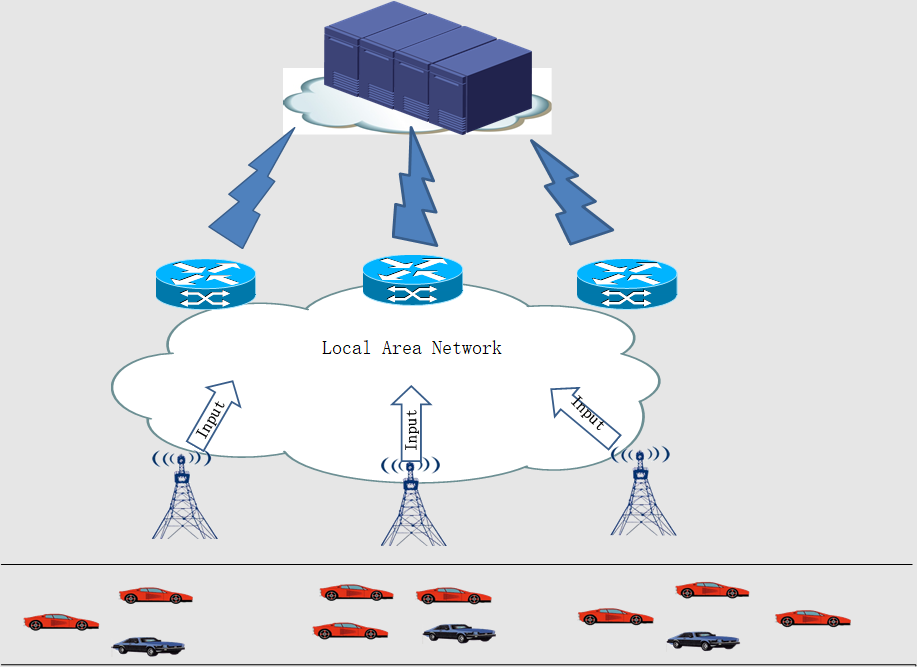
\includegraphics[scale=0.4]{4.png}
\caption{Overall architecture of a fog-cloud computing system}
\label{fig:label}
\end{figure}

\begin{table}[h]
	\centering
	\begin{tabular}{p{1cm}p{5cm}}
	\hline
	Symbol & Definition \\\hline
	$i$ & index of fog devices\\
	$j$ & index of cloud devices\\
	$M$ & size of the fog device set $\mathcal{M}$\\
	$N$ & size of the cloud server set $\mathcal{N}$\\
	$r,R,\mathcal{R}$ & index, number, set of RSUs\\
	$u,U,\mathcal{U}$ & index, number, set of vehicles\\
	$\lambda_{ij}$    & traffic rate dispatched from fog device $i$ to cloud server $j$\\
	$y_j$             & workload assigned to cloud server $j$\\
	$f_i$	          & CPU frequency of fog device $i$ \\
	$L$               & total input from all RSUs\\
	$X$               & workload allocated for fog computing\\
	$Y$               & workload allocated for cloud server\\
	$P$               & power consumption\\
	$D$               & delay\\
	$v_i$             & service rate for fog device $i$\\
	$f_j$             & machine CPU frequency at cloud server $j$\\
%	$\sigma_j$        & on/off state of cloud server $j$\\
	$b_{ur}$               & $2 \times 1$ dimension matrix\\      
	$n_j$             & machine number in cloud server $j$\\
	$d_{i,j}$         & communication delay from fog device $i$ to cloud server $j$\\\hline
	\end{tabular}
	\caption{Symbols}
\end{table}


\subsection{System Model}
We concern to minimize the consumption with an guaranteed delay in our system model. We are mainly concerned about the following parts.

\textit{1) Power Consumption of Fog Device:} The computation power consumption of fog device \textit{i} can be calculated by a function of the CPU frequency $f_i$.The function must be a monotonic increasing function.For simplicity but without loss of generality,the power consumption $p_i^{fog} $ of device $i$ is defined as followsA
$$ p_i^{fog} \triangleq a_if_i^2+b_if_i+c_i $$
,where $f_i$ is the CPU frequency of fog device $i$ and $a_i,b_i,c_i$ are non-negative,pre-determined parameters. 

\textit{2) Communication Delay of Fog Device:} We assume that it is a queueing system for the fog device to process requests. For the device $i$ , the computation delay $D_i^{fog}$ which includes waiting time and service time is 
$$ D_i^{fog} \triangleq \frac{1}{v_i-x_i}$$
,where $x_i$ is the arrival rate and the $v_i$ is the service rate.

\textit{3) Power Consumption of Cloud Server:} As mentioned before, each cloud server hosts numerous computing machines. We simply assume that the CPU frequencies of these machines are equal in a cloud server. The number of machines in cloud server $j$ is denoted by $n_j$. In this situation, the power consumption of cloud server $j$ can be expressed as the product of the  machine consumption value and the number of machines in server $j$. We approximate the power consumption value of each machine in server $j$ by a function of CPU frequency $f_j$:$P^{mh} = A_jf_j^p+B_j$, where $A_j$ and $B_j$ are positive constants, and $p$ is in the range of 2 to 3. 

Hence, the power consumption $P_j^{cloud}$ of the cloud server $j$ can be calculated by multiplying the number of machines and the value of each machine power consumption.
$$P_j^{cloud} = n_j\left(A_jf_j^p+B_j\right)$$

\textit{4) Communication Delay of Cloud Server:} The delay of cloud server can be obtained by $D_i^{cloud} = t_{queue}+t_{service}$. We model the system as a queueing network, and the cloud can be modeled as $M/M/n$ queue. Thus, the total computation delay of cloud server is given by
$$D_j^{cloud} \triangleq \sigma_j\left[\frac{C\left(n_j,y_jK_j/f_j\right)}{n_jf_j/K_j-y_j} + \frac{K_j}{f_j}\right]$$ ,where the $K_j$ denotes the average cycle of requests and the $C\left(n_j,y_jK_j/f_j\right)$ is Erlang’s C formula \cite{17}.

\textit{5) Communication Delay of Transmission:}
Communication delay of dispatch: We use $w_{ij}$ to record the bandwidth from fog device $i$ to the cloud server $j$. Let the binary variable $\lambda_{ij}$ denote the traffic rate dispatched from the fog device $i$ to the cloud server $j$. The communication delay of dispatch is 
$$ D_{ij}^{dis} \triangleq \lambda_{ij} \frac{data\ size}{w\cdot \log_2(1+\frac{S}{N})}.$$

Communication delay of vehicles and RSUs: For vehicle $u$ and RSU $r$ we get the time consumption through the V2I mode as $D_{ur}^{v2i} = t_{up}+hi_{ur}*t_{backhaul}$. In the V2V mode, it can be described as $ D_{ur}^{v2v} = t_{up}+hv_{ur}^{j}*t_{v} $ ,where $t_v$,$hv_{ur}^j$ denote a one-hop V2V delay and the V2V relay hops that are required in transmitting the input data to the j-hop-away RSU,respectively.
The delay of VANET and RSUs can be similarly given as 
$$
D_{ur}^{trans} = b_{ur} \cdot \begin{bmatrix}
D_{ur}^{v2v} \\
\\
D_{ur}^{v2i}
\end{bmatrix} 
$$
,where $b_{ur}$ is either $\begin{bmatrix}
0 & 1 
\end{bmatrix} $ or $\begin{bmatrix}
1 & 0 
\end{bmatrix} $ which depends on which mode to choose. 

\textit{6) Power Consumption of transmission:} The physical network infrastructures mainly include road side units (RSUs),Routers(fog layer) and vehicles. Let $\mathcal{R}$ and $\mathcal{U}$  be the sets of RSUs and vehicles ,respectively, where $\mathcal{R}=\left\{1,\ldots,R\right\}$,$\mathcal{U}=\left\{1,\ldots,U\right\}$.There are two transmission modes from vehicles to RSUs. The first is direct V2I mode and the other is V2V predictive-
mode transmission. We can compute the power consumption of the task from vehicle $u$ to RSU $r$ in V2I mode as 
$$p_{ur}^{v2i} = p_{upload} + hi_{ur} \cdot p_{backhaul},$$ 
where the $hi_{ru},p_{backaul}$ donate the number of hops from the original RSU to the destination RSU and the cost for transmitting the output data across one road segment,respectively. 

Furthermore, unlike the RSU access service that is provided by some infrastructures, the V2V communication is always self-organized by running vehicles and power costs are much less than V2I mode. The power consumption of the task in this mode from vehicle $u$ to RSU $r$ can be described as $p_{ur}^{v2v} = p_{upload}+hv_{ur}^j \cdot p_{v}$  ,where $hv_{ur}^j$ denotes the V2V relay hops that are required in transmitting the input data to the j-hop-away RSU. Recall that $j$ is the hops of the upload destination RSU away from the vehicle's current position. Thus,$j>1$ means the vehicles adopt the predictive-mode transmission.%
In general, the consumption of transmission is  
$$ P_{ur}^{trans} = b_{ur} \cdot \begin{bmatrix}
p_{ur}^{v2v} \\
\\
p_{ur}^{v2i}
\end{bmatrix} $$.

\subsection{Constraints}

Assuming that L denote the total requests input from all RSUs. These requests should be sent to a N set of fog devices. Thus, it satisfies 
$$
L \triangleq \sum_{i \in \mathcal{N}} l_i
$$

Let $\mathit{X}$,$\mathit{Y}$ respectively denote the workload for fog computing and cloud computing. Then we have
$$
\left\{
\begin{array}{lr}
\mathit{X} \triangleq \sum_{i \in \mathcal{N}} x_i &  \\
\mathit{Y} \triangleq \sum_{j \in \mathcal{M}} y_j. &
\end{array}
\right.
$$

The requests from RSUs can be devided into two parts, which are processed by fog devices or cloud servers,respectively. To be more specific, the corresponding relationship is as following.

Workload balance constraint for each cloud server
\begin{equation}
\sum_{i \in \mathcal{N}} \lambda_{ij} = y_j \qquad \forall j \in \mathcal{M}
\end{equation}

Workload balance constraint for each fog device
\begin{equation}
l_i - x_i = \sum_{j \in \mathcal{M}} \lambda_{ij} \qquad \forall i \in \mathcal{M}
\end{equation}
Obviously , from (6)(7) we can obtain 
\begin{equation}
L = X+Y
\end{equation}

\textit{4)WAN Bandwidth Constraint:} For the transmission path from fog device $i$ to the fog server $j$, let $\lambda_{ij}^{max}$ denotes the max bandwidth capacity. Moreover, these transmission paths do not overlap with each other. The constraint of WAN communication bandwidth is as follows:
\begin{equation}
0 \leq \lambda_{ij} \leq \lambda_{ij}^{max} \qquad \forall i \in \mathcal{N}; \quad \forall j \in \mathcal{M}
\end{equation}
In V2V transmission mode, the data is transmitted to the j-hop-away RSU by vehicles. In order to meet low delay, the hop number $j$ should be no more than a threshold.
\begin{equation}
j \leqslant j_{max}
\end{equation}
\subsection{Problem Formulation}
We propose our model toward trade-off on power consumption and delay in vehicular fog computing system. we want to minimize the power consumption ,meanwhile ensuring the low-delay	The vehicular end experienced delay consist of the computation delay and transmission delay.
The total delay of the proposal model is defined as
\begin{gather}
D^{sys} \triangleq \sum_{i \in \mathcal{N}} x_i \cdot D_i^{fog} + \sum_{j \in \mathcal{M}} y_j \cdot D_j^{cloud} + \notag \\
 \sum_{i \in \mathcal{N}}\sum_{j \in \mathcal{M}} D_{ij}^{dis}+ \sum_{u \in \mathcal{U}}\sum_{r \in \mathcal{R}} D_{ur}^{trans}.
\end{gather}
The power consumption consists of the fog layer and the cloud layer, which is shown as below.
$$
P^{sys} \triangleq \sum_{i \in \mathcal{N}}x_iP_i^{fog} + \sum_{j \in \mathcal{M}} y_jP_j^{fog}+\sum_{u \in \mathcal{U}}\sum_{r \in \mathcal{R}} P_{ur}^{trans}.
$$

We consider the problem of minimizing the power consumption ,as mentioned before, while guaranteeing the max tolerance delay $\overline{D}$ for vehicular end. Then we have the PP
\begin{equation}
\begin{split}
%
\min_{x_i,y_j} p^{sys}  \\  
s.t.\left\{
\begin{array}{lr}
D^{sys} \leq \overline{D} &  \\
(1)-(4). &
\end{array}
\right.
%	
\end{split}
\end{equation}


The exact solution of the above problem consists in solving the above problem as  a mixed integer non-linear
programming (MINLP) problem, which is a NP-Hard problem. Thus, in case of large scale applications, the problem solving time is unacceptable.
\section{Solutions}
We divide the whole system into two parts: the front end and the back end. The front end consists of vehicles and RSUs. The cost of front end is mainly consumption and delay of communication between vehicles and RSUs and we want to minimize the $D_{ur}^{trans}$ and $P_ur^{trans}$. We adopt the predictive combination-mode scheme to solve the above problem. The back end,however, contains the fog nodes and cloud servers. We proposed a deep learning model to minimize the back-end cost as follows.
\subsection{Greedy Algorithm}
We propose a simple and well-understood greedy algorithm\cite{18}. In the greedy algorithm, the requests are queued and we successively process each request. We choose the server,which has the minimum power consumption under the constraints conditions,for the request in each step. For each request, we place it to the current optimal position. And we get the total power consumption  and delay of these requests. The pseudocode of the algorithm is given in the Algorithm 1. Although the result obtained by greed algorithm is not the global optimal solution, it will not be too bad.  In the simulation section we compare our model with the cloud-only model using the greedy algorithm. 
\begin{algorithm}[htb]   
\caption{Greedy algorithm}   
\label{alg:Framwork}   
\begin{algorithmic}[1] %这个1 表示每一行都显示数字  
\REQUIRE ~~\\ %算法的输入参数:Input  
The set of requests  $\mathit{Q}=\left\{q_1,q_2,\dots,q_m \right\} $;\\  
The status list of servers $S=\left\{s_1,s_2,s_3,\dots,s_n \right\}$;\\ 
The tolerable total delay $D$
\ENSURE ~~\\ %算法的输出:Output  
The minimum of power consumption ;\\
The serial number of server nodes for requests \\ 
\STATE $serial\_list \leftarrow \left\{ \right\}$
\STATE $sum \leftarrow 0$
\STATE $\overline{D} \leftarrow \frac{D}{\left|Q\right|}$
\FOR{each $q \in Q$}
\STATE $minimum \leftarrow +\infty$
\FOR{each $s_i \in S$}
\STATE $q \rightarrow s_i$
\IF{satisfy the constraint $\overline{D}$}
\STATE  $p \leftarrow $calculate power consumption of $q$
\IF{$p<minimum$}
\STATE $minimum \leftarrow p$
\STATE $no \leftarrow i$
\ENDIF
\ENDIF 

\ENDFOR
\STATE $sum \leftarrow sum+minimum$ 
\STATE $serial\_list \Leftarrow no $
\STATE Update the status info of server $i$
\ENDFOR
  
\RETURN $sum,serial\_list$; %算法的返回值  
\end{algorithmic}  
\end{algorithm}  

\subsection{Deep Learning Model}
\subsubsection{Input and Output Design}
Our considered system model is depicted in Fig 1. In our model, we totally have $n$ optional edge computing nodes and cloud servers to handle requests from the front-end. Therefore, each node holds a record of the number of requests and average power consumption in the last $\mathit{H}$ periods. We adopt these records as the input of our deep learning model \cite{19} and our considered deep CNN structure is shown in Fig 2. In order to train our CNN model, labeled data (i.e.many sets of $(x,y)$) are required to perform supervised training.

The deep CNN comprises two main components,respectively,the feature extraction and classification parts. In the feature extraction part,convolution layers are used to filter the low level features of the input data while the pooling layers are used to reduce the size of features and parameters ,and speed up calculation in the network. Features of the input data can be extracted from the convolution and pooling layers. Based on these extracted features, the fully connected layer compute the output results of the classification.

The deep learning structure is utilized to compute the candidate service provider. Therefore, we choose the server number as the output in our deep learning model.Thus, the output value is in the range of $[0,N-1]$.


\begin{figure}[h]
\centering
\subfigure[considered deep CNN structure]{
\begin{minipage}[b]{0.5\textwidth}
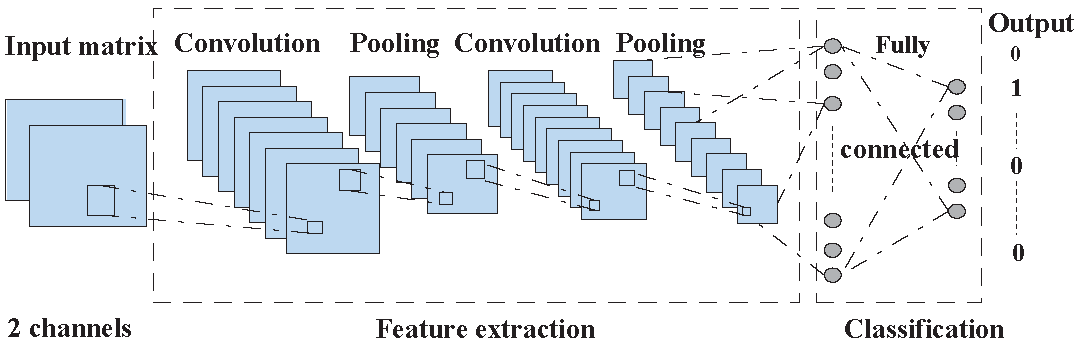
\includegraphics[width=1\textwidth]{a.png}
\end{minipage}
}
\subfigure[input characterization]{
\begin{minipage}[b]{0.5\textwidth}
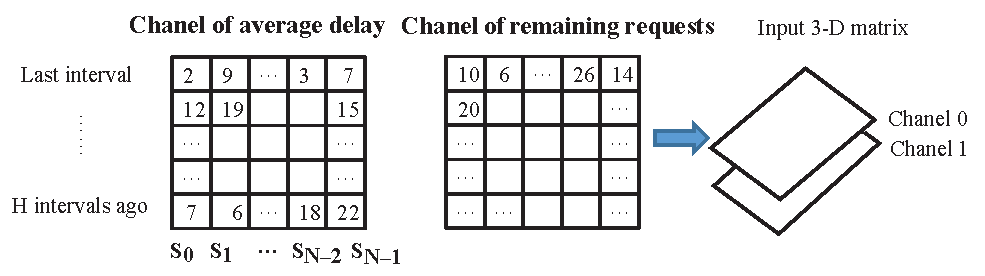
\includegraphics[width=1\textwidth]{b.png}
\end{minipage}
}
 \caption{Our input characterization for the deep CNN} 
 \label{fig:label}
\end{figure}

\subsubsection{Initialization Phase}
As described in Input and Output Design, we need labeled data to train our CNN model. In the initialization phase, we need to obtain the labeled data. The purpose of the initialization phase is to get the labeled data which consist of the input vector and the corresponding output result \cite{20}. It is best to train our CNN model with the global solution of formula 12. However, the time complexity of solving the optimal solution is $O(n^m)$, which is not tolerated. We choose a compromised method to get the labeled data. We adopt a heuristic algorithm to obtain the near-optimal solution.  As shown in algorithm 2, the simulated annealing(SA) algorithm mainly consists of two key step: generate a new solution with some functions and accept the new solution with a certain probability \cite{21}. We take the solution of our greedy algorithm as the initial solution in SA algorithm.

The SA algorithm iterates $L$ times at a certain temperature to search the global optimal solution. In the searching process, the SA algorithm poor solution with the probability of $\exp(-\frac{\triangle t}{T})$, where $\Delta t$ is the evaluation difference between the new solution and the origin. With the SA algorithm, we can obtain the labeled data for our CNN model. The input of our CNN model is the records information of servers in last $H$ intervals. Thus, we obtain the record information of servers and the corresponding offloading result.

\begin{algorithm}[!h]   
\caption{Simulated Annealing Algorithm}   
\label{alg:Framwork}   
\begin{algorithmic}[1]
\REQUIRE ~~\\ %算法的输入参数:Input  
The set of requests  $\mathit{Q}=\left\{q_1,q_2,\dots,q_m \right\} $;\\  
The list of servers $S=\left\{s_1,s_2,s_3,\dots,s_n \right\}$;\\ 
The tolerable total delay $D$ \\
\ENSURE ~~\\
The minimum of power consumption ;\\
The serial number of server nodes for requests \\ 
\STATE Initial temperature T,temperature threshold $T^{'}$, iterations L
\STATE Initial solution\\ $s \leftarrow Greedy  Algorithm(Q,S,D)$
\WHILE{$T>T'$}
\REPEAT
\STATE  Displace some requests from high performance to low performance randomly
\IF{Delay<D}
\STATE Get new solution $s'$
\ENDIF
\STATE calculate $\Delta t = C(s')-C(s)$
\IF{random [0,1] < $\mathrm{e^{\frac{-\Delta t}{T}}}$}
\STATE accept new solution $s'$
\STATE record serial\_list,$C(s')$
\ENDIF
\IF{satisfy final condition}
\RETURN $C(s')$, serial\_list
\ENDIF
\STATE$K \leftarrow K+1$
\UNTIL{K==L}
\STATE $T = \alpha\cdot T$, where $\alpha$ is an attenuation factor
\ENDWHILE
\RETURN $C(s')$, serial\_list
\end{algorithmic}  
\end{algorithm}  
\subsubsection{Training Phase}
In the training phase, we use the data obtained in initialization phase to train the CNN model. The training phase consists of two step: initializing the parameters in our designed CNN and fine-tuning the parameters with BP(back-propagation) algorithm. It is necessary to initial the parameters,which is benefit to accelerate the convergence speed. The CNN parameters are initialized by normal Gauss distribution with a mean value of zero. 

For feed-forward neural network, parameter optimization depends on the error back-propagation. The optimization phase can be done by the stochastic gradient descent(SGD) algorithm or the Adam algorithm. Since the Adam algorithm is adaptive, we choose adam as the optimization algorithm in our training phase as shown in Algorithm 3. In the training phase, we take the cross-entropy cost function as the loss function. Thus, the output is a scalar which is the neuron index of the maximum value in the output layer.
\begin{algorithm}[!h]   
\caption{Training Algorithm}   
\label{alg:Framwork}   
\begin{algorithmic}[1]
\REQUIRE ~~\\
$(x,y)= \left\{(x^{(t)},y^{(t)})|t=1,2,\dots,m \right\}$
\ENSURE  ~~\\
$\theta$
\STATE initial $\theta$ randomly
\FOR{$(x_i,y_i) \in (x,y)$}
\STATE predict = forward($x_i$,$\theta$)
\STATE loss = loss\_fun(predict,$y_i$)
\STATE loss.backward()
\STATE update $\theta$
\ENDFOR
\end{algorithmic}  
\end{algorithm} 

\subsubsection{Running Phase} 
In running phase all servers need to record the number of received requests and average power consumption over a period of time and send these records to edge computing nodes. In this way, each edge node can take these records as an input to calculate the offloading result. However, it is possible to obtain an inappropriate result which doesn't meet the constraints in the CNN running phase. In such situation, we take the greedy algorithm as an compensation.


\section{PERFORMANCE EVALUATION}
In order to validate the performance of our model, we conduct the simulations on the front end and back end. The related parameters in the simulation is shown as table 2.
\begin{table}[h]
	\centering
	\begin{tabular}{p{3cm}p{3cm}}
	\hline
	Variable & Value \\\hline   
	$N$             & 20\\
	$M$             & 5\\
	$n_j$           & $20\sim25$ \\
	$f_i$           & $4.5\sim5.5$ \\
	$f_j$           & $2.5\sim3.5$ \\
	request packet size & $5\sim15MB$ \\
	request need cycles & $0.7\sim0.9$ \\\hline
	\end{tabular}
	\caption{parameters}
\end{table}

As mentioned before, we used the predictive combination-mode model in the front-end. Before sending requests, broadcast packets are sent to ask the nearby vehicles or RSU for the back-end processing delay. With the delay result and vehicle speed, vehicles can calculate the arriving RSU when the requst returns. In the combined-model, the power consumption and delay of V2I,V2V model are estimated to choose the optimal model. In the simulation, we assume that vehicles are travelling in a straight line and the simulation result is shown as figure 3

\begin{figure}[ht] 
  \centering 
  \subfigure[house]{ 
    %\label{fig:subfig:a} %% label for first subfigure 
    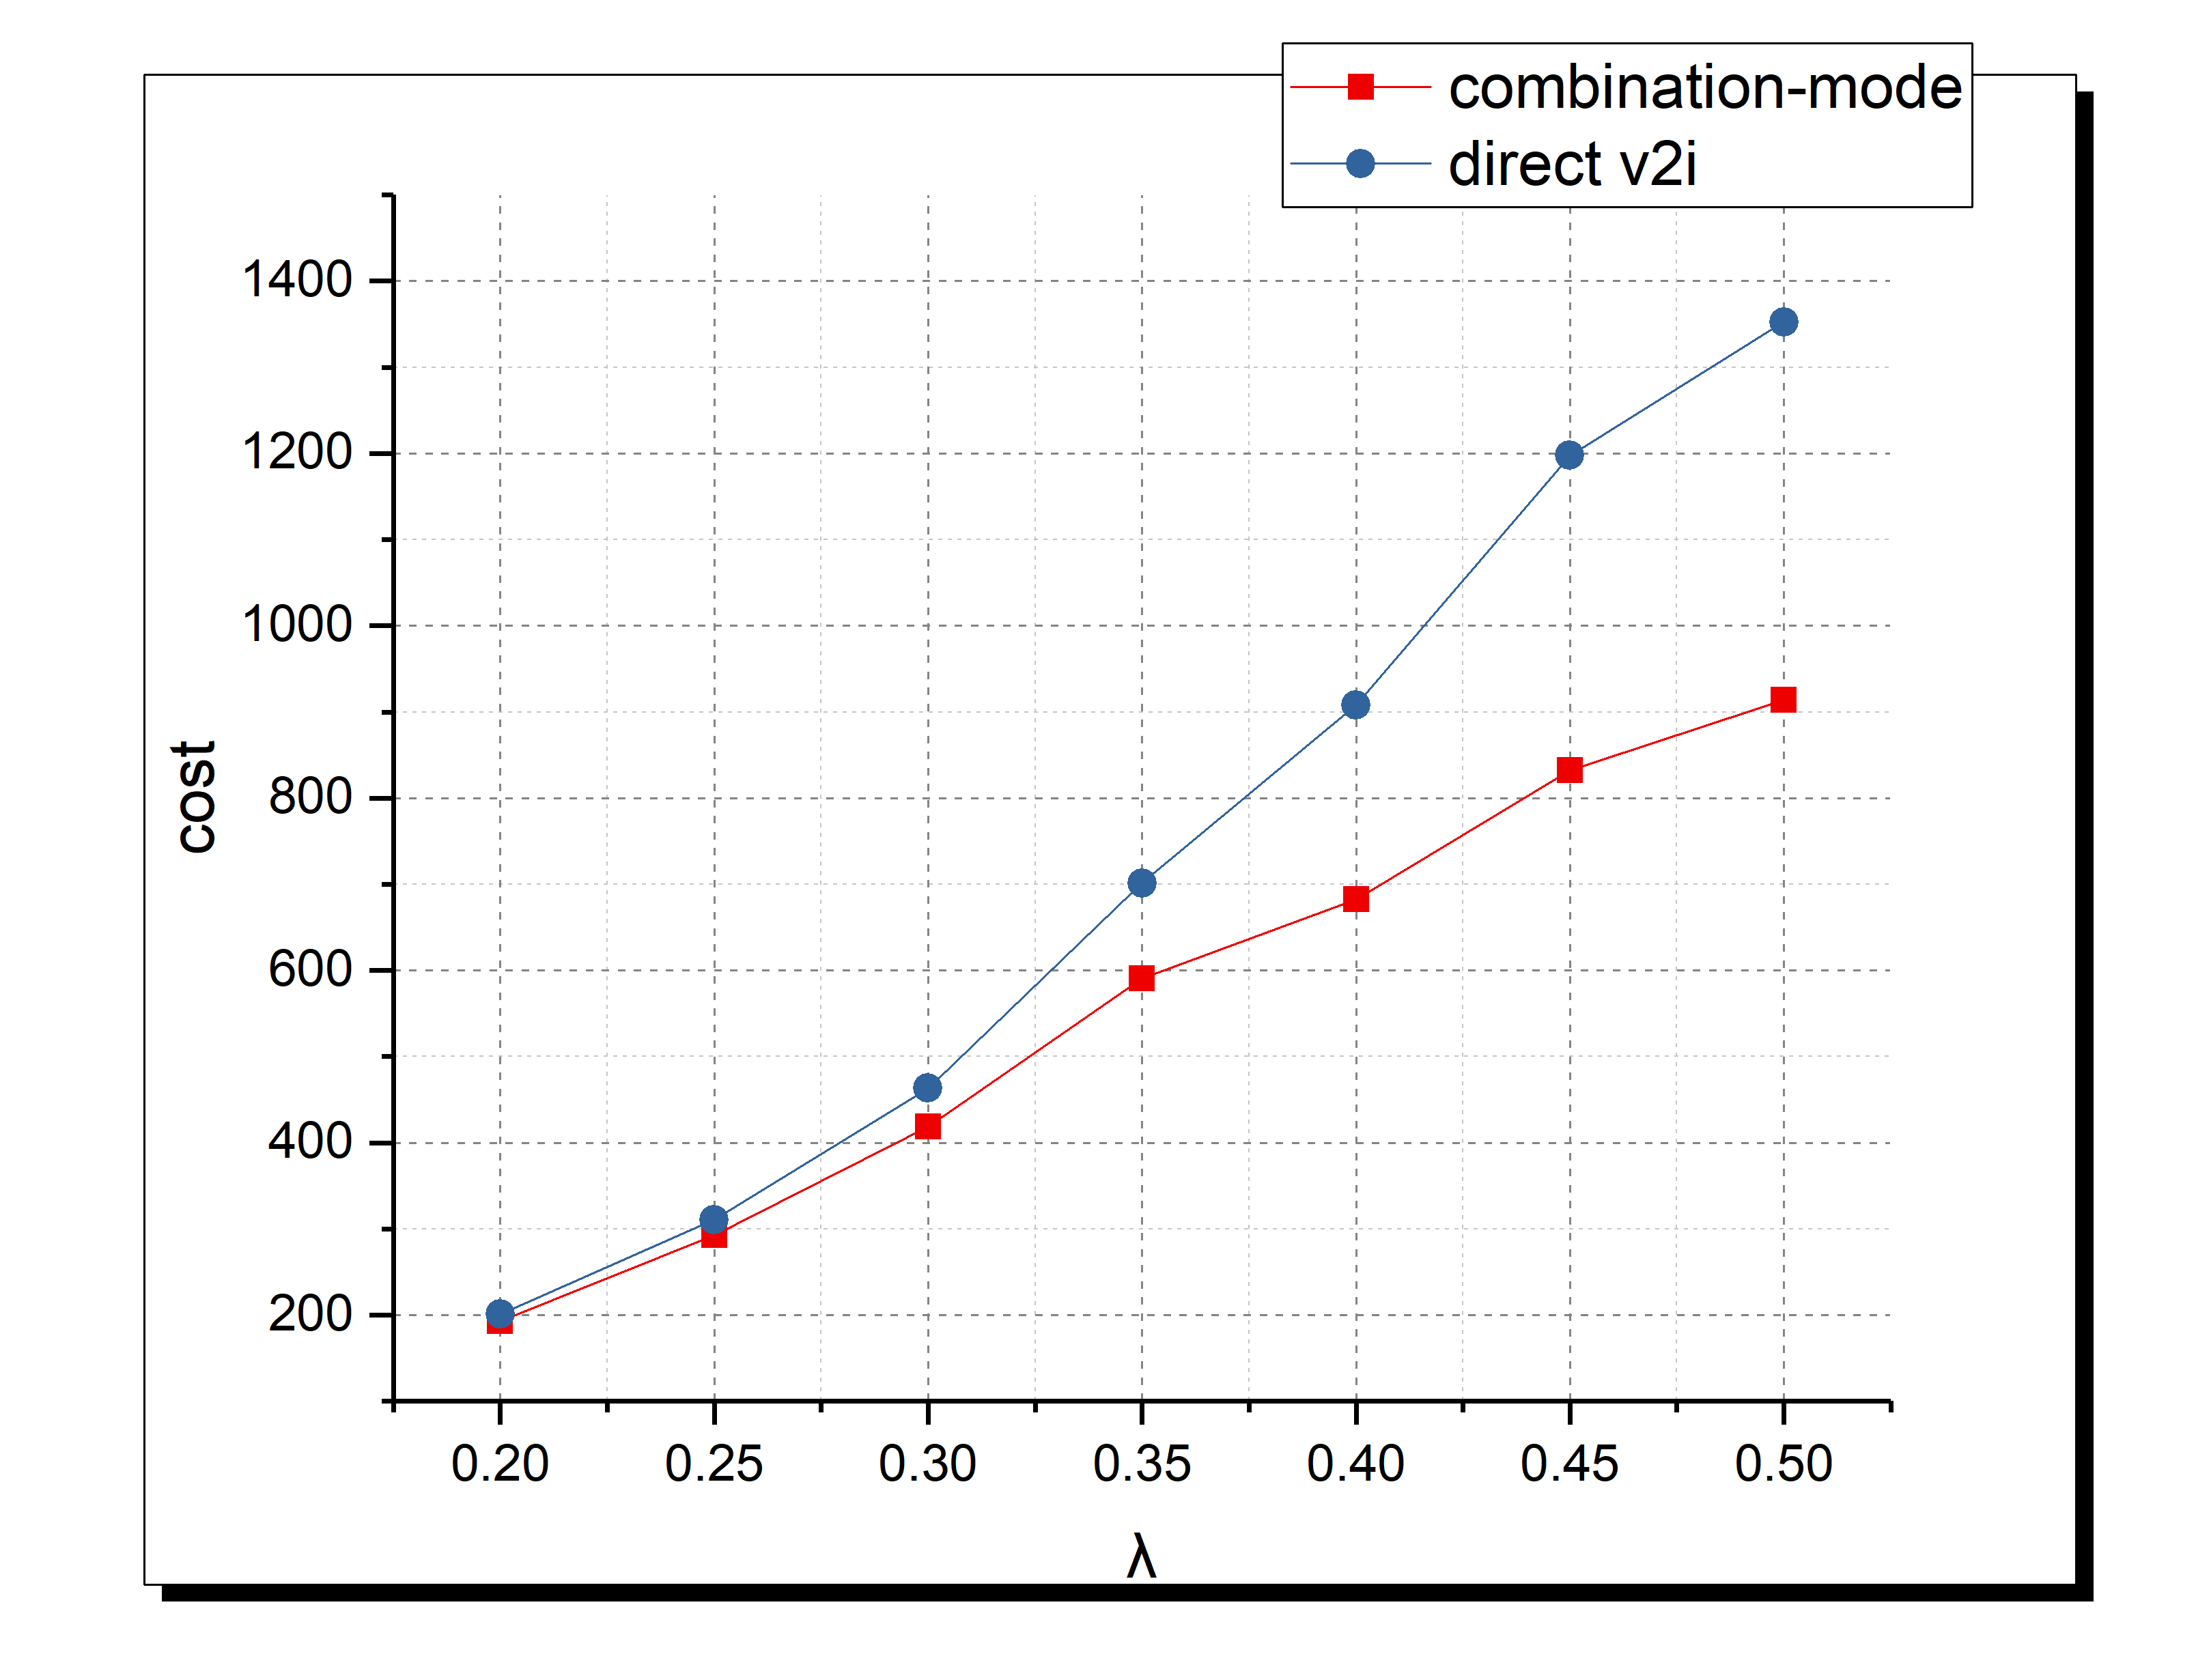
\includegraphics[width=0.22\textwidth]{./c.png} 
  } 
  \subfigure[hotel]{ 
    %\label{fig:subfig:b} %% label for second subfigure 
    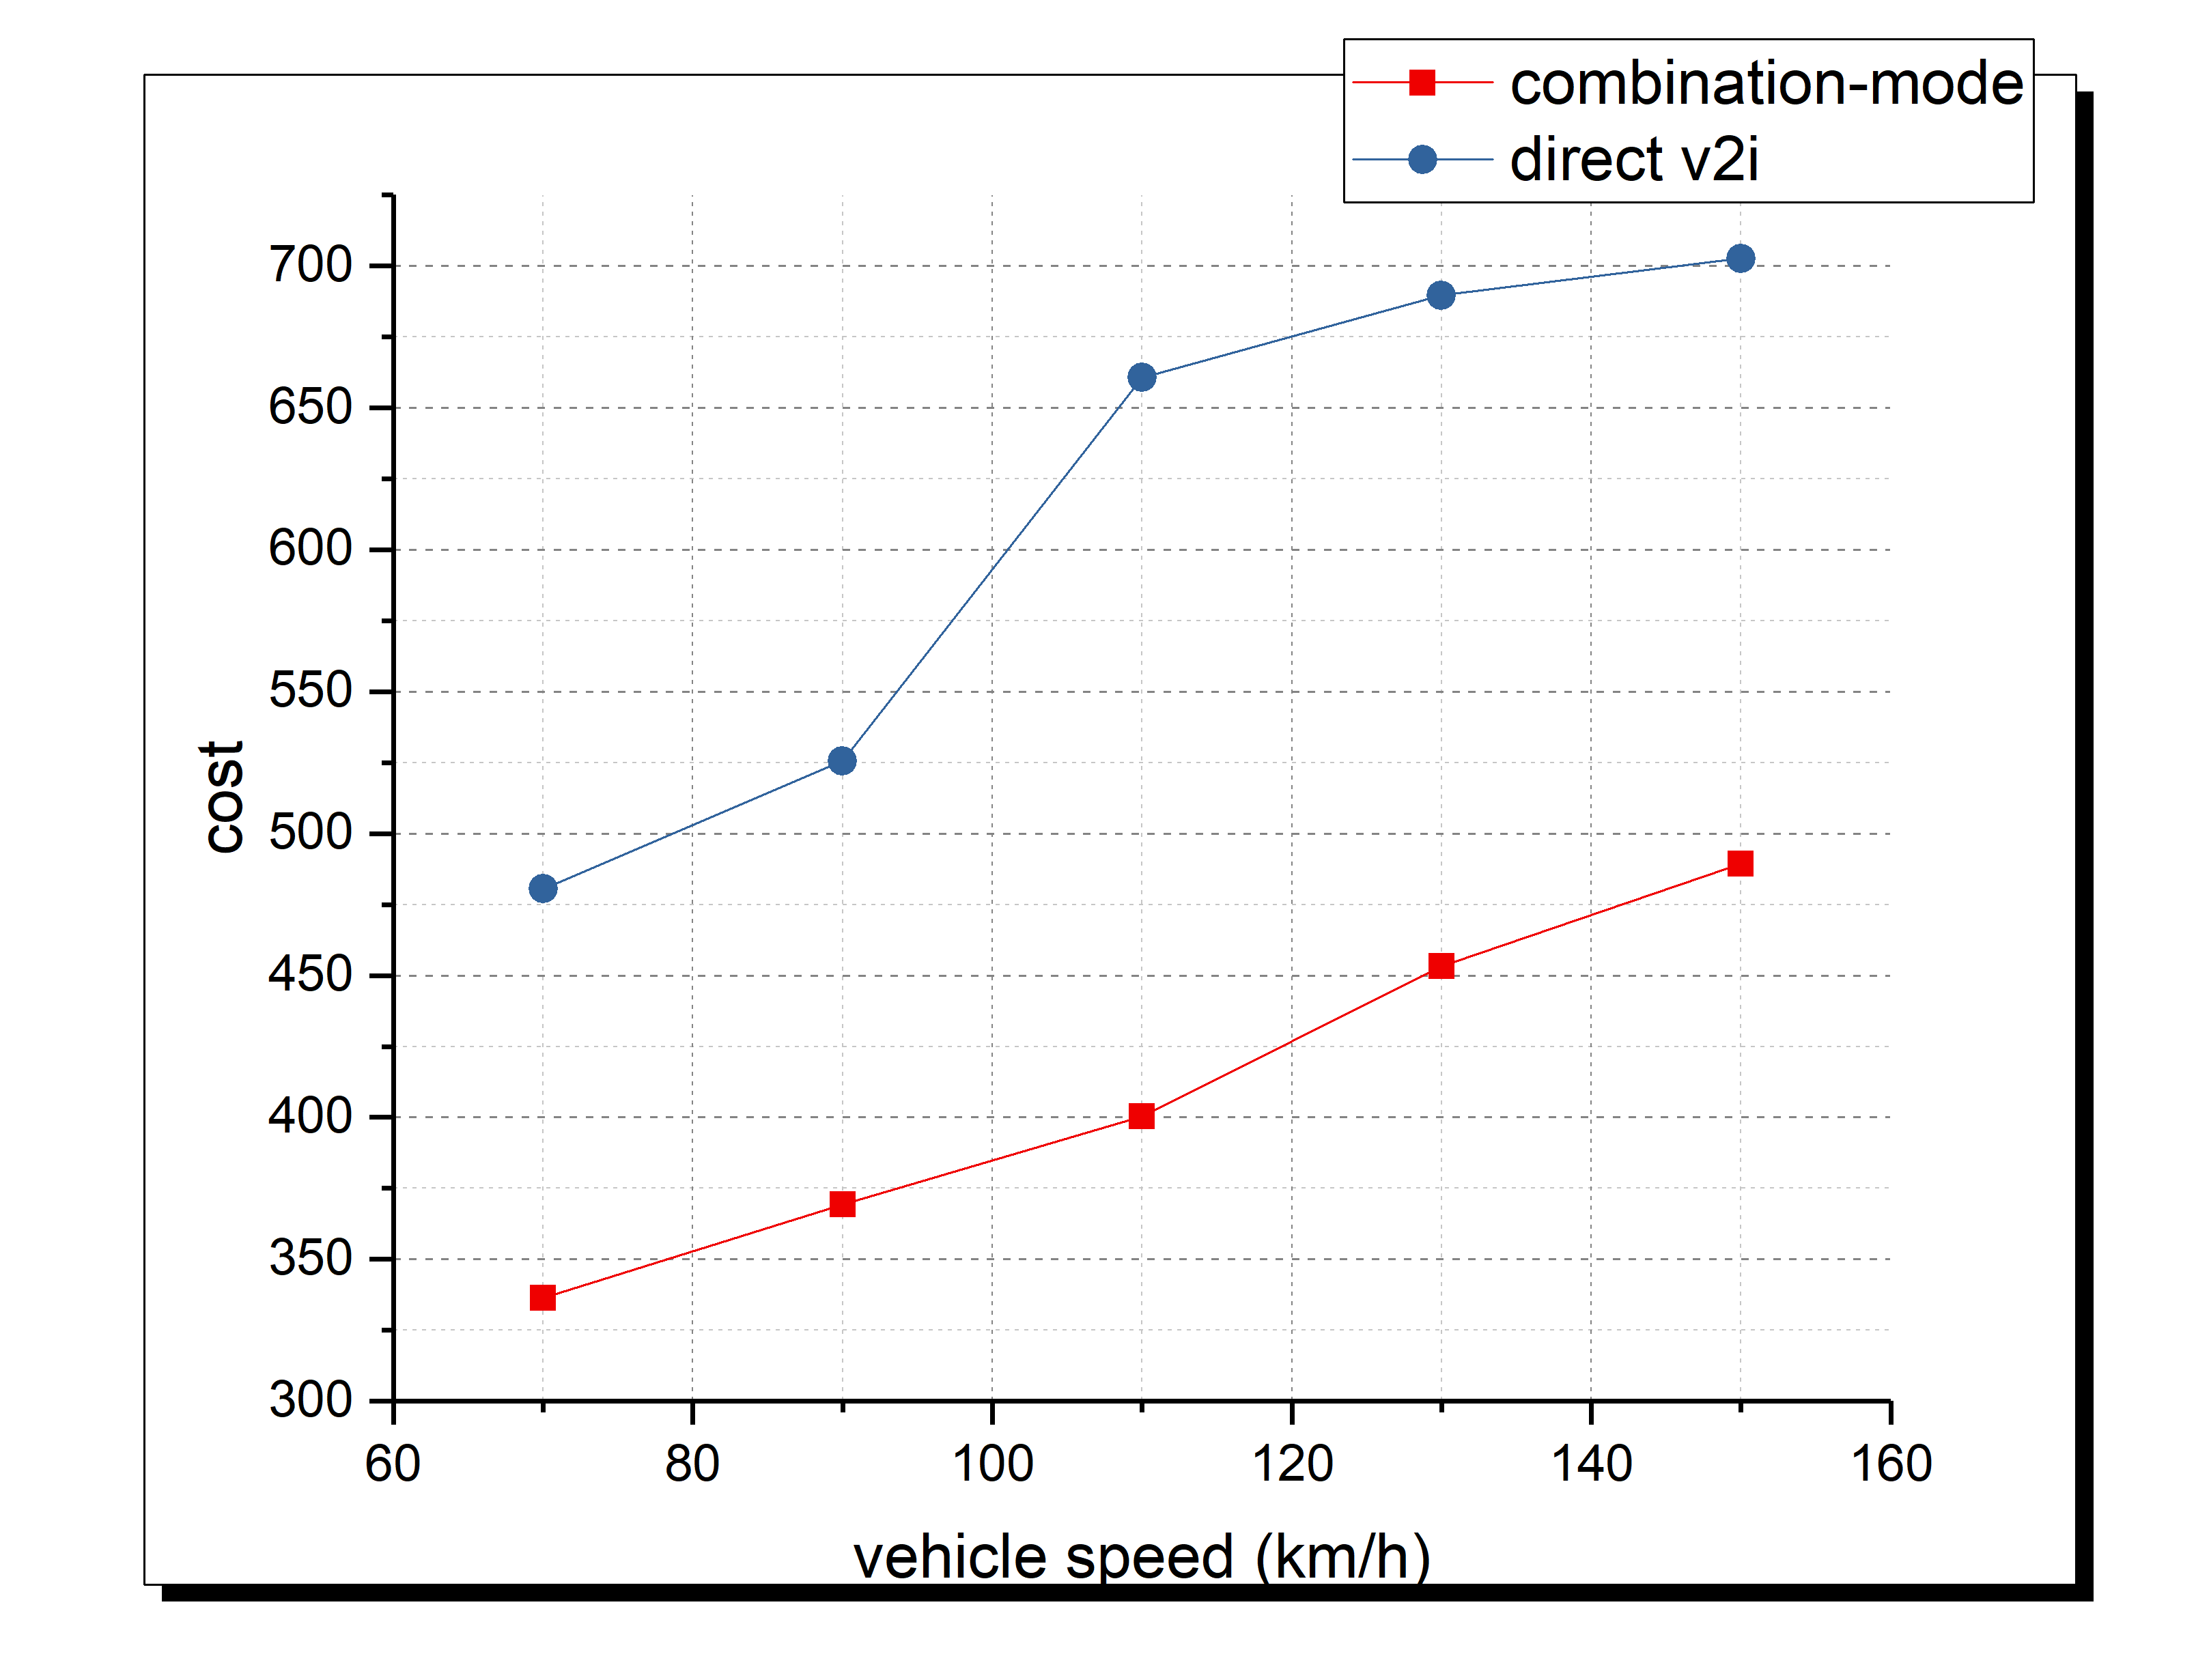
\includegraphics[width=0.22\textwidth]{./d.png} 
  } 
  \caption{} 
  %\label{fig:subfig} %% label for entire figure 
\end{figure}

Figure 3 illustrates the performance of cost with different vehicle speed and vehicle density. With higher vehicle speed, the cost of the combined-mode is much lower than the V2I mode. For the V2I mode, the cost grows significantly with the speed of 100 to 120. That is because with that speed most vehicles are at the edge of RSU coverage when the request returns. Therefore, when the speed exceeds a threshold, the vehicles will drive into another RSU. The cost of V2I mode will increase significantly. In addition, the optimization effect of combined-mode is obvious with a heavy traffic density. With a heavy traffic density, the delay and power consumption of each hop in V2V mode reduced a lot. 

In order to validate the performance of fog-cloud model. We compare the performance of fog-cloud model with cloud-only and fog-only mode. 
\begin{figure}[htp]
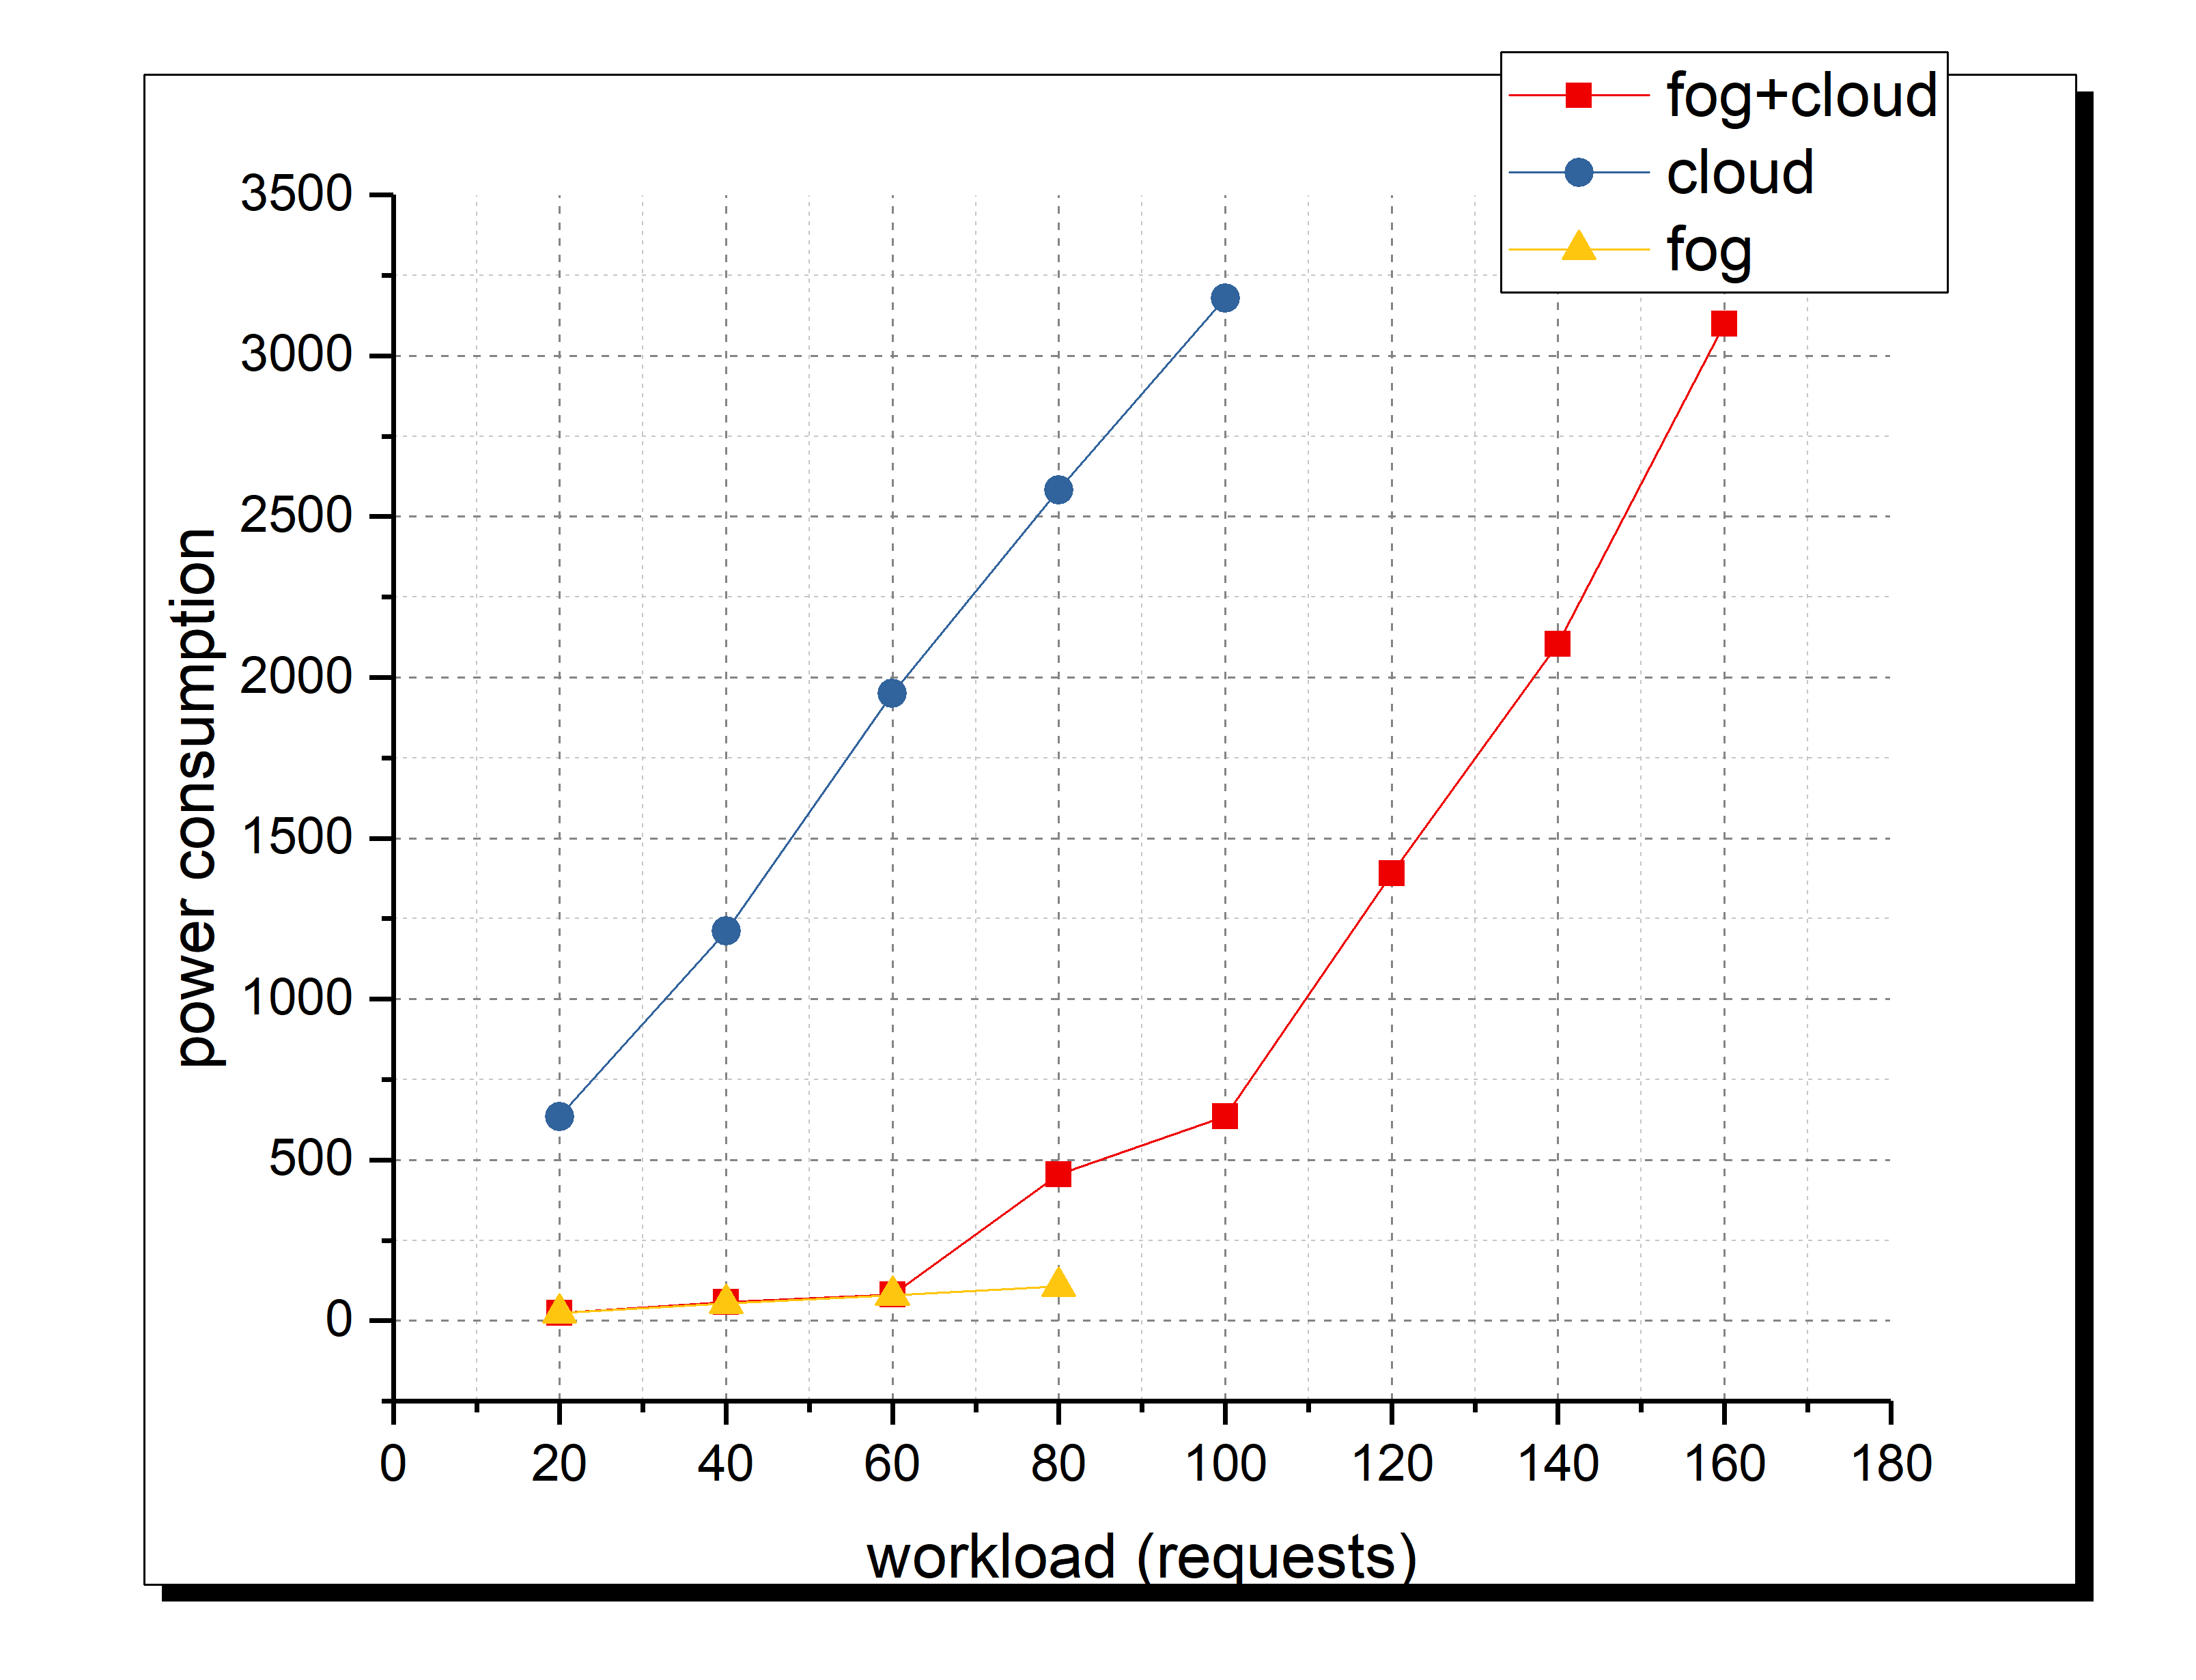
\includegraphics[width = 0.5\textwidth]{e.png}
\caption{Comparison of energy consumption}
\end{figure}

As shown in figure 4, the power consumption of fog-only is extremely low but no more than 80 requests can be handled at one time. The fog-cloud model is much better than the cloud-only model with the workload of 20 to 100. The power consumption of the fog-cloud model is almost the same as that of fog-only model with the workload of 20 to 80. In such situation, the workload of fog layer is not saturated and most requests are processed by the fog node. When the workload is more than 100, the fog layer reaches saturation,after which the power consumption growth trend in the fog-cloud model is similar to the cloud-only model.

Moreover, the maximum workload of fog-cloud model is much larger than the other two models. Figure 5 illustrates the performance of delay with different workload. The average delay of fog-cloud model is less than 1.5 seconds. Whereas, in the other two model the average delay is fast-growing. 
\begin{figure}[htbp]
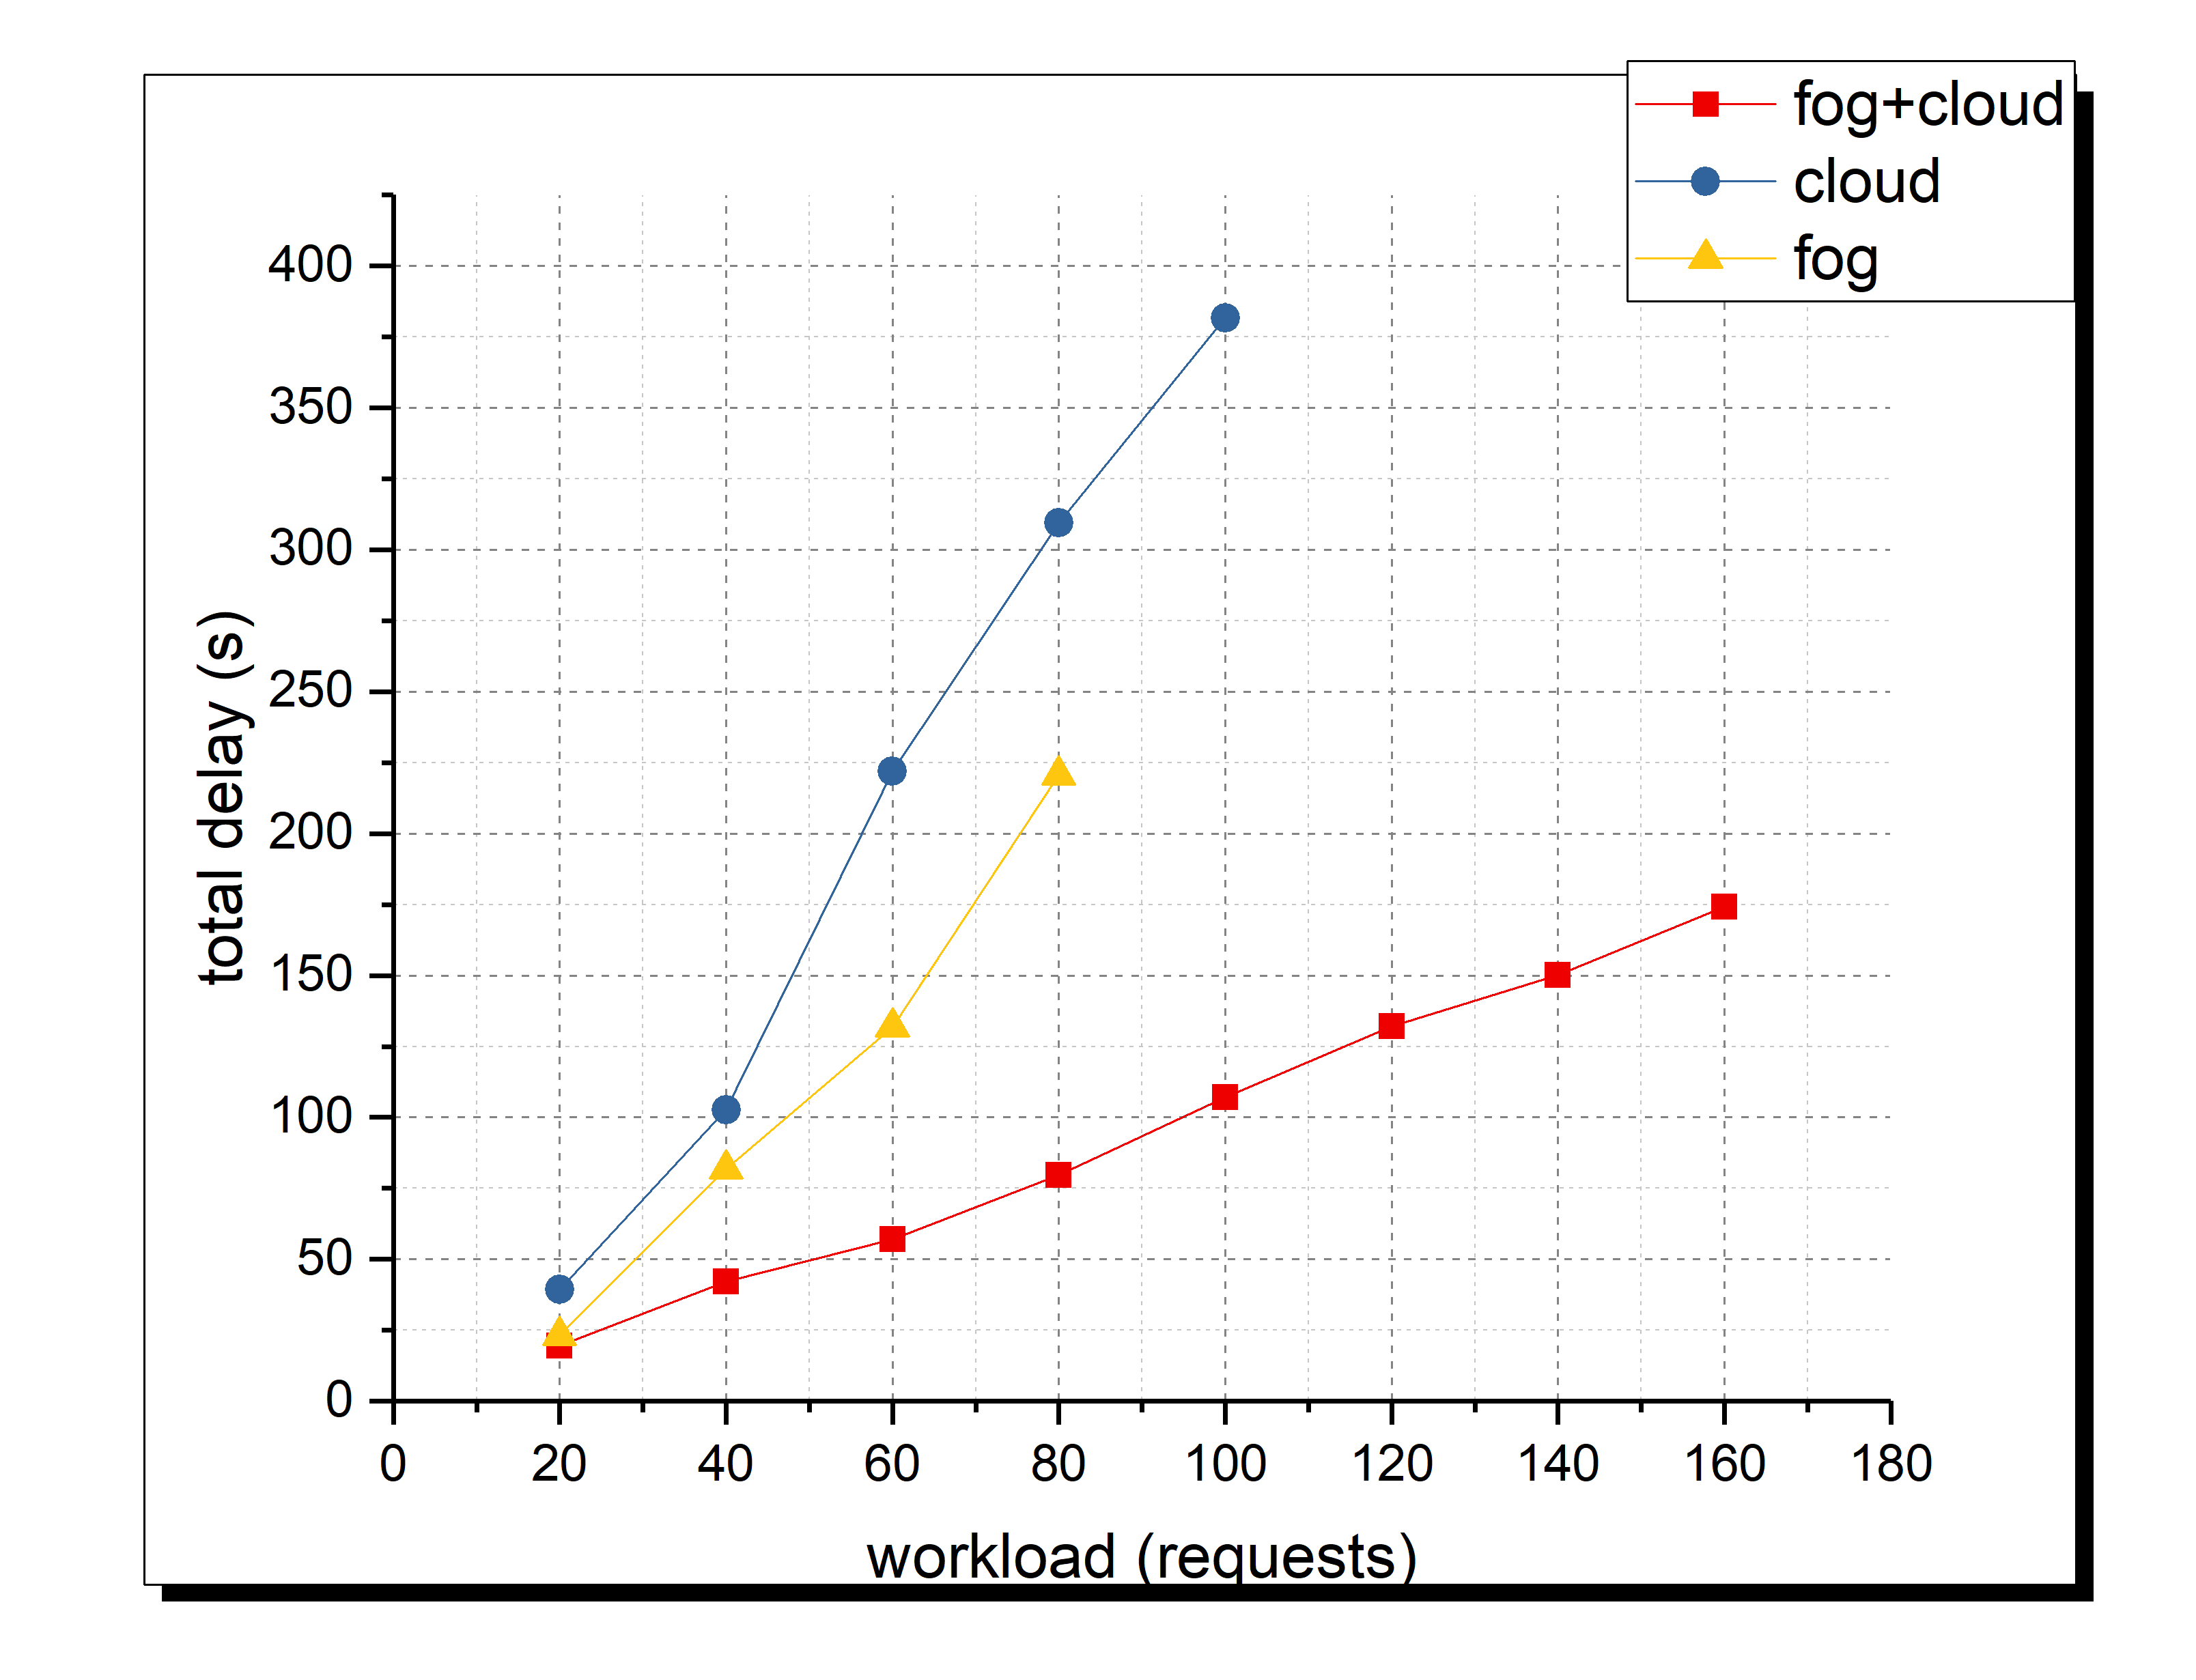
\includegraphics[width = 0.5\textwidth]{f.png}
\caption{Comparison of delay}
\end{figure}

As mentioned before, we take the last H interval records of servers as input in CNN model. The CNN model in the simulation is shown in figure 6. We take the records of last four $\Delta t$ intervals as input, where $\Delta t$ is equal to 2 seconds. In each interval $\Delta t$, the average number of request is 50. The training data is obtained by SA algorithm in 20 consecutive intervals. 
\begin{figure}[htbp]
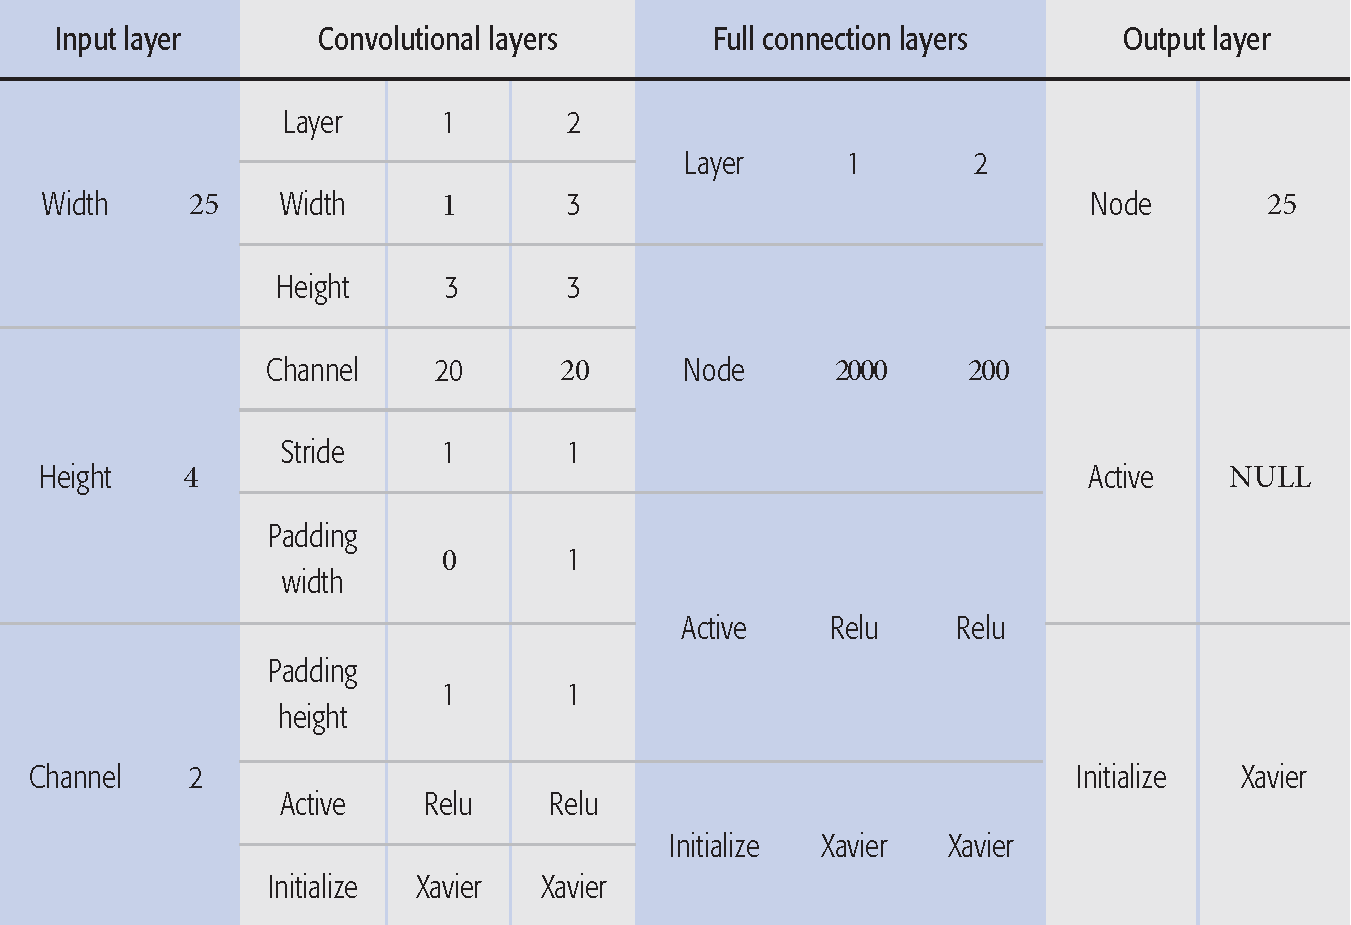
\includegraphics[width = 0.5\textwidth]{g.png}
\caption{CNN model structure}
\end{figure}

After training, we obtain the offloading result of requests by CNN model. The power consumption of different algorithm is shown in figure 7. Our deep learning model can effectively reduce the computational complexity in the running phase and the performance is much better than the greedy algorithm
\begin{figure}[htbp]
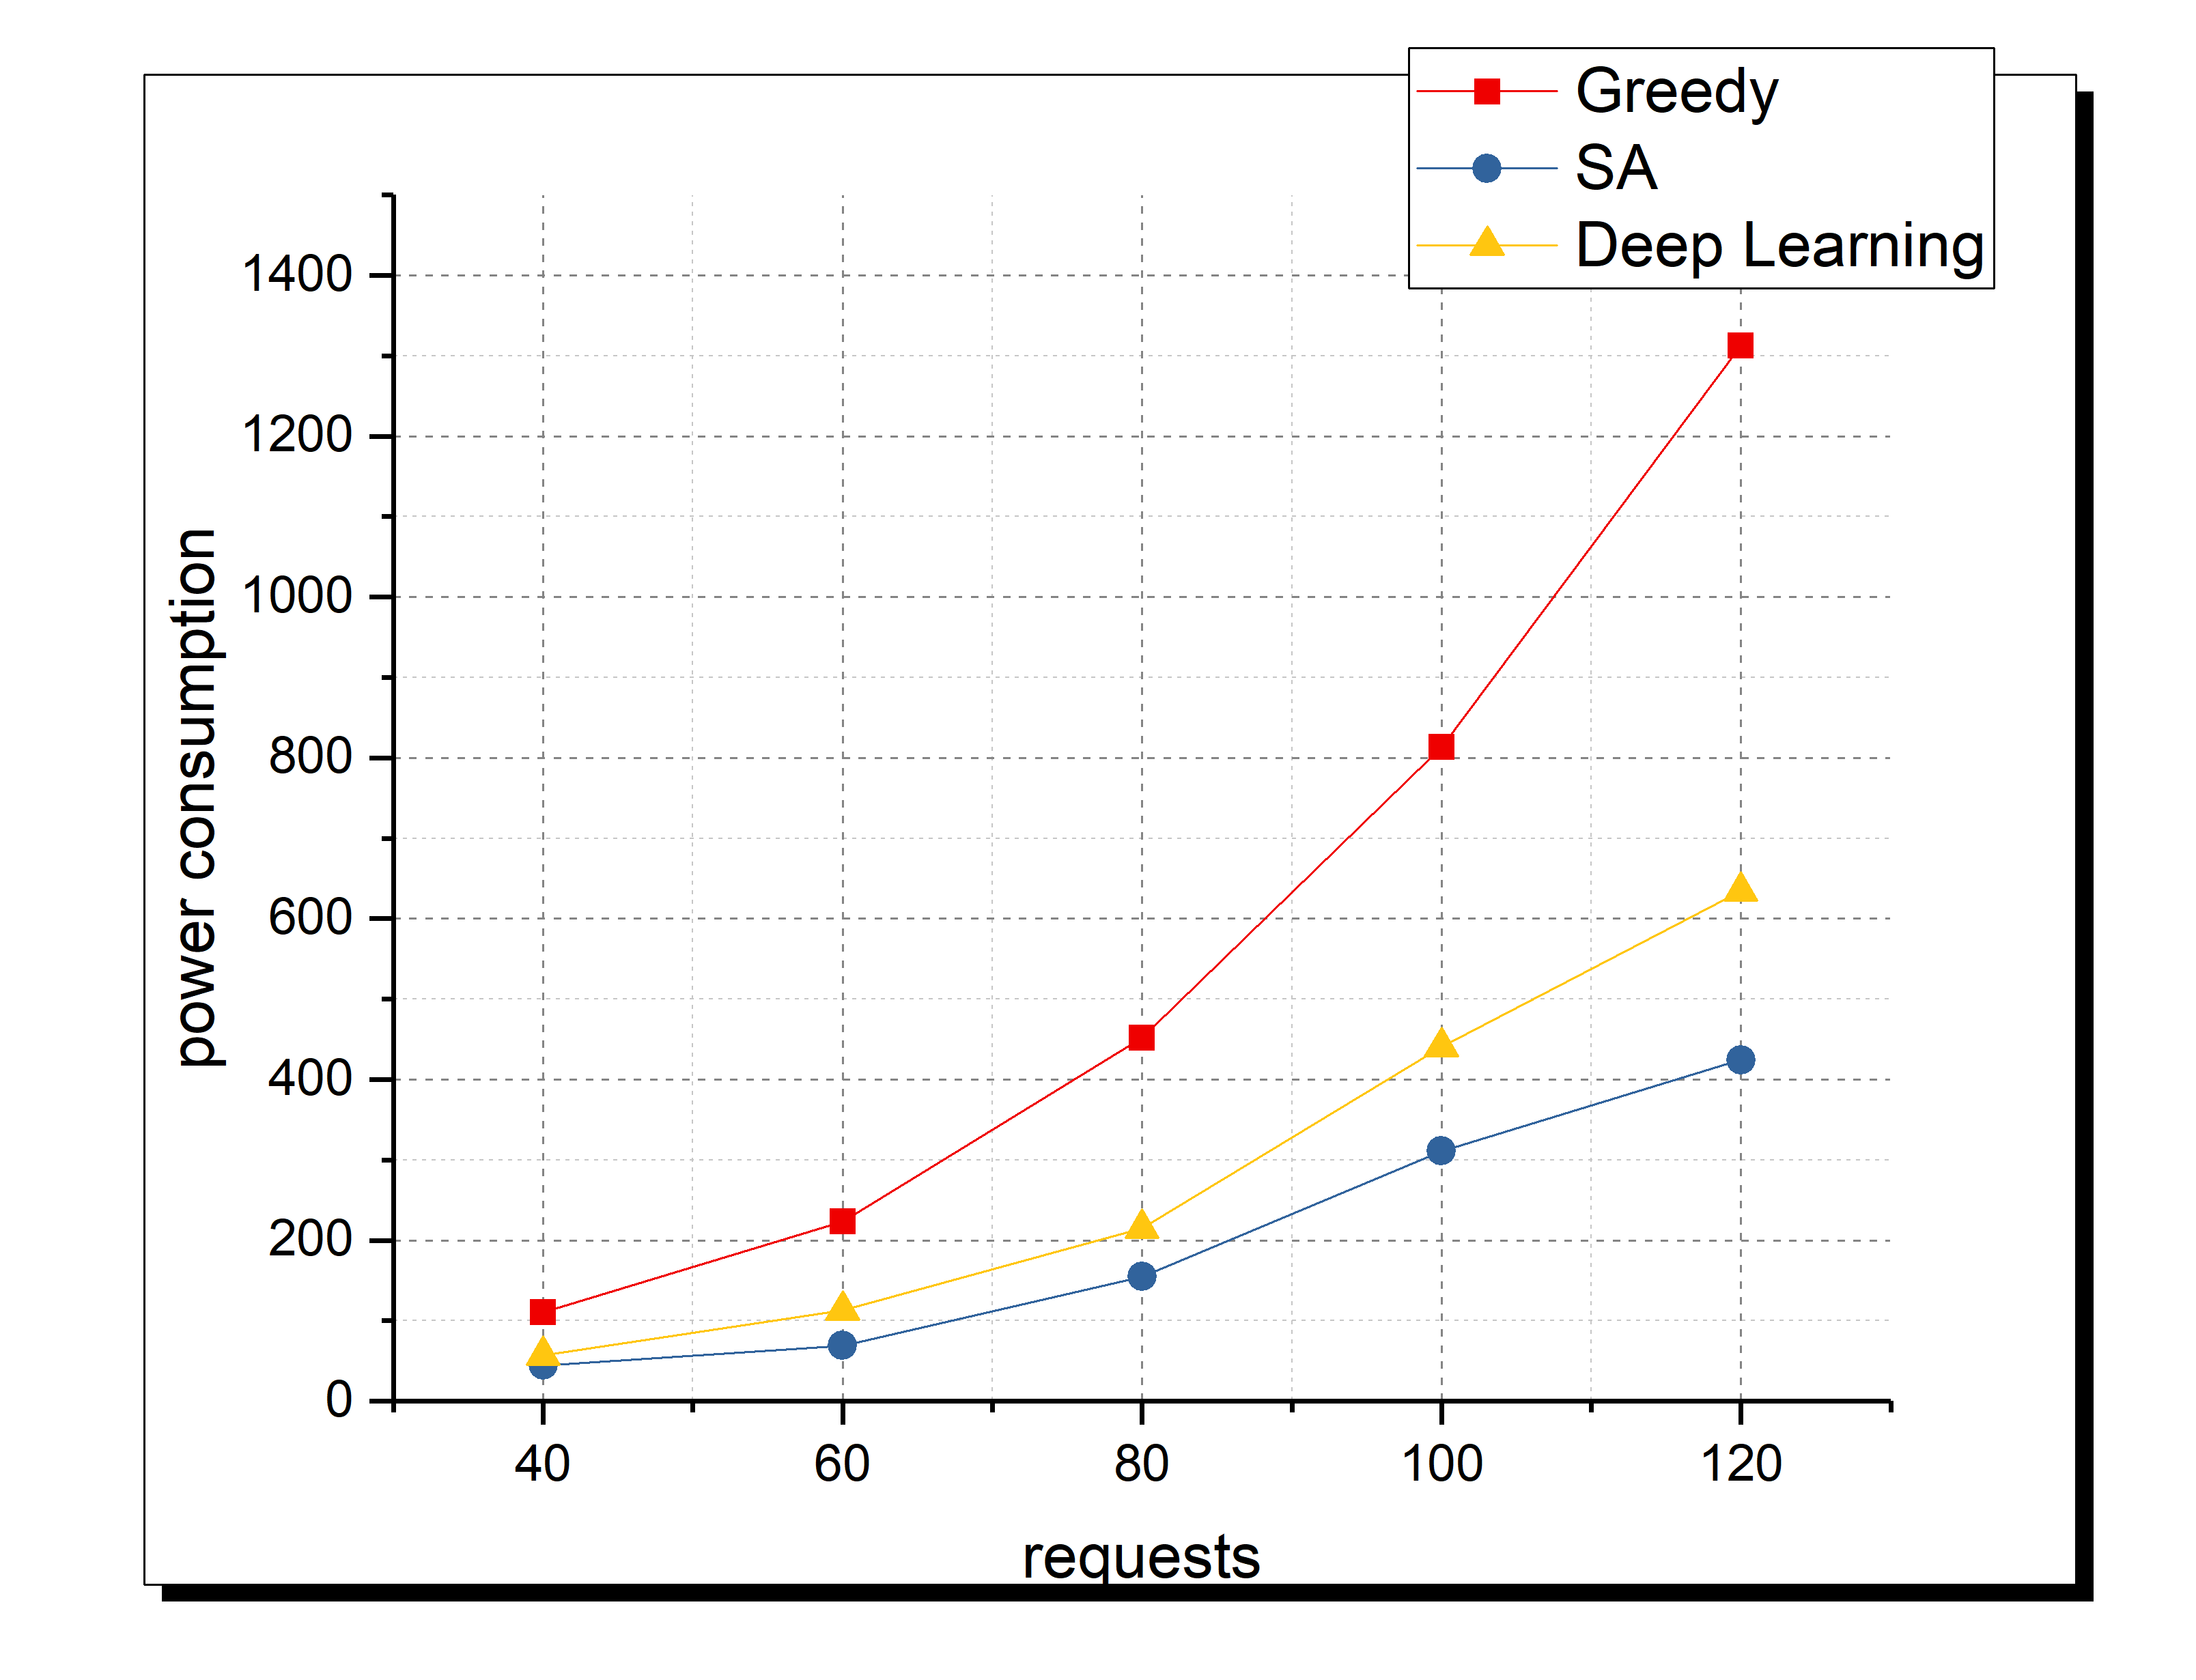
\includegraphics[width = 0.5\textwidth]{h.png}
\caption{Power Consumption of Deep Learning and other algorithm}
\end{figure}


\section{Conclusion}
In this paper,we propose a fog-cloud model based on deep learning ,which is a feasible solution to minimize the power consumption and delay in the back-end. The offloading optimization problem is formulated in our proposed model.For the fog nodes, they can be modeled as M/M/1 in queueing theory. For the cloud servers, they can be modeled as M/M/n queue. In addition, we propose a predictive combination-mode model to minimize the cost in front-end. In the simulation, we can draw the conclusion that the fog-cloud model shows good performance compared to the cloud-only mode or the fog-only mode. Our deep learning model is an approximate approach to solved the formulated problem.



\bibliographystyle{ieeetr}
\bibliography{bare_jrnl}




% that's all folks
\end{document}


